\documentclass{ituthesis}
\usepackage[]{hyperref}
\usepackage[]{float} 
\usepackage[]{csquotes} 
\usepackage[]{graphicx} 
\usepackage[font={scriptsize}]{caption} 
\usepackage[]{subcaption} 
\usepackage[]{mdframed}
\usepackage[]{ntheorem} 
\usepackage[]{fixltx2e} 
\usepackage[]{mathpartir} 
\usepackage[]{syntax} 
\usepackage[utf8]{inputenc} 
\usepackage[]{listings} 
\usepackage[scaled=.8]{beramono} 
\usepackage[backend=bibtex, style=authoryear]{biblatex}
\bibliography{report.bib}

\lstset{basicstyle=\ttfamily}

\definecolor{constructor-color}{RGB}{155,187,89}
\definecolor{type-color}{RGB}{142,180,227}
\definecolor{declared-var-color}{RGB}{192,80,77}
\definecolor{local-var-color}{RGB}{230,185,184}
\definecolor{literal-color}{RGB}{179,162,199}

\newcommand{\ttconstructor}[1]{\textcolor{constructor-color}{\texttt{#1}}}
\newcommand{\tttype}[1]{\textcolor{type-color}{\texttt{#1}}}
\newcommand{\ttdec}[1]{\textcolor{declared-var-color}{\texttt{#1}}}
\newcommand{\ttvar}[1]{\textcolor{local-var-color}{\texttt{#1}}}
\newcommand{\ttliteral}[1]{\textcolor{literal-color}{\texttt{#1}}}

\theoremstyle{break}
\theorembodyfont{}
\newtheorem{exmp}{Example}
\newtheorem{alg}{Algorithm}

\newenvironment{asideblock}
  {\begin{mdframed}[style=0,%
      leftline=false,rightline=false,leftmargin=2em,rightmargin=2em,%
          innerleftmargin=0pt,innerrightmargin=0pt,linewidth=0.75pt,%
      skipabove=7pt,skipbelow=7pt]\small}
  {\end{mdframed}}

\settitle{The Practical Guide to Levitation}
\setauthor{Ahmad Salim Al-Sibahi}
\setsupervisor{Dr. Peter Sestoft}
\setextrasupervisor{David R. Christiansen}
\setdate{September 1, 2014}

\begin{document}
%\selectlanguage{danish}

\frontmatter

\thetitlepage
\newpage

\chapter*{Abstract}
Goal: Implementation of levitation in a realistic setting, with practical performance benefits.
\blockquote{DISCLAIMER: This is a draft and as such is incomplete, incorrect and can contain grammatical errors.
Although I claim originality of this report, many underlying ideas are based on current work in the scientific community which will be correctly attributed
when the work is complete.}

\cleardoublepage
\setcounter{tocdepth}{1}
\tableofcontents

\mainmatter
\midsloppy
\sloppybottom
\chapter{Introduction}
\label{cha:Intoduction}
\section{Context}
\label{sec:Context}
Algebraic datatypes such as Boolean values, lists or trees form a core part of modern functional programming.
Most functions written work directly on such datatypes, but some functions like structural equality or pretty printing (see Example~\ref{exmp:prettyprint}) don't directly dependent on the datatype itself.
Therefore, writing such functions for each different datatype becomes a repetitive exercise.
In fact it is possible to write an algorithm over the structural definition of the datatype, which the computer then could use to derive an actual function for each particular datatypes.

\begin{exmp}
  Pretty printing an element of any algebraic data type follows a very simple procedure:
  \begin{enumerate}
    \item Print the name of the constructor
    \item Iterate over the constructor arguments and pretty print them, with each argument surrounded by parentheses if necessary
    \begin{enumerate}
      \item If the argument is a recursive reference to the type itself, then call this procedure recursively (starting at point 1).
      \item If the data element is of another type, then
      \begin{enumerate}
        \item Find the correct pretty printing function for that type
        \item Pretty print the field using the found function
      \end{enumerate}
    \end{enumerate}
  \end{enumerate}
  \label{exmp:prettyprint}
\end{exmp}

Enter the world of \textit{generic programming} where the target datatype is the one describing the structure of other datatypes, often called the \textit{description}\label{kw:desc}.
While generic programming sounds promising, it is usually seen as an aspect of Haskell\,\autocite{haskell98} that is challenging to use by ordinary programmers. To represent the description, it is often required to use special language extensions\,\autocite{magalhaes2010generic,Jansson:1997:PPP:263699.263763} and the programming style tends to require different abstractions than when writing ordinary programs.

%A tiny bit of history here?
However, in dependently-typed languages such as Idris\,\autocite{brady2013idris} or Agda\,\autocite{norell2009dependently} it is possible to create a correct description using ordinary datatype definitions\,\autocite{benke2003universes}.
Furthermore, \textcite{Chapman:2010:GAL:1863543.1863547} show that it is possible to build a self-supporting closed type system which is able to convert these descriptions to ordinary types (creating so-called \textit{described types}), while still being powerful enough to describe the description datatype itself.
In such system, generic programming is just a special case of ordinary programming.

%\subsection{The Importance of Genericity in Dependently-typed Languages}
%\label{sub:TheImportanceofGenericityinDependently-typedLanguages}
%\textit{The similarity of structure and various slightly-different indexing of types.}


\section{Problem definition}
\label{sec:ProblemDefinition}
The current work on generic programming in dependently-typed languages presents both elegant and typesafe ways to represent the structural descriptions of datatypes.
Furthermore, it allows the programmer to save both time and boilerplate code while reducing mistakes by using ordinary programming techniques to do generic programming.

However, the state of the art is heavily theoretically oriented, which might lead to some challenges when a system needs to be developed with a practical audience in mind.
First of all, multiple description formats are often presented, sometimes even in the same paper, which might not be particularly attractive in a practical setting.
Secondly, there has been little work done on how to integrate such descriptions in languages which contain features such as type classes and proof scripts.
Finally, datatypes synthesised from descriptions create large canonical terms; thus, both type checking and runtime performance are very slow.
In the end, if an efficient and easily usable framework for programming with described types could be implemented successfully, it would save programmers both the time and effort required to write repetitive functions.

\section{Aim and scope}
\label{sec:AimandScope}
The aim of this research is to provide a practical and efficient implementation of described types in Idris.
This project has three primary goals.

The first goal is to find a good definition of the description that supports many common datatypes.
I mainly seek to reuse some of the existing work, and not to further develop underlying type theory to support more complex inductive families; neither will I focus on supporting all language features of Idris such as implicit arguments and codata definitions.

The second goal is to present realistic examples using generic functions working on described types. 
This mainly includes implementing functions that can be used to derive type class instances, and a Scrap Your Boilerplate-style (SYB) library for generic querying and traversal.

The final goal is to describe how partial evaluation and related techniques can be used to optimise the generic functions with regards to specific descriptions in order to achieve acceptable performance.
This includes using techniques such as polyvariant partial evaluation\,\autocite{Jones:1993:PEA:153676} and constructor specialisation\,\autocite{Mogensen:1993:CS:154630.154633}. %Elaborate when I know more about PE\ldots

\section{Significance}
\label{sec:Significance}
The main contributions of this thesis are:

\begin{itemize}
  \item an example-based tutorial for understanding described types in the context of a practical programming language, namely Idris;
  \item an generic implementation of common operations such as decidable equality, pretty printing and functors, which can be used to provide default implementations to type class methods;
  \item a discussion of the challenges that arise when trying to implement a SYB-style generics library in dependently typed languages;
  \item optimisation techniques based on partial evaluation for reducing runtime size and time overhead for described types and accompanying generic functions;
  \item metrics showing that generic programming using described types is a viable option to reduce boilerplate without significant cost in performance.
\end{itemize}
\section{Overview}
\label{sec:Overview}

The report is structured as follows. Chapter~\ref{cha:GenericProgramming} presents an introduction to described types specifically focusing on recent developments using dependently-typed programming languages.
Chapter~\ref{cha:PartialEvaluation} presents an overview of techniques for partial evaluation of functions and specialisation of datatypes. Chapter~\ref{cha:LevitatingIdris} discusses specifically how I implemented described types in Idris and continues with practical examples in Chapter~\ref{cha:PracticalExamples}.
Chapter~\ref{cha:OptimizingIdrisforFlight} presents the optimisations that can be made in order to improve the runtime performance of described types and generic functions. Evaluation of the results happens in Chapter~\ref{cha:Evaluation} comparing the performance of generic implementations to hand-written ones.
Finally, Chapter~\ref{cha:Discussion} discusses the challenges that still lie ahead and concludes the effort.
\chapter{Generic programming}
\label{cha:GenericProgramming}
\section{The generic structure of inductive data types}
\label{sec:TheGenericStructureofInductiveDataTypes}
\subsection{Anatomy of a datatype}
\label{sub:AnatomyofaDatatype}
To build an intuition that will be useful in understanding descriptions, let us first start by looking closely at how datatypes are structured.
Recall from Page~\pageref{kw:desc} that a description is a data value representing the structure of a particular datatype.
Figure~\ref{fig:anatomydatatype} presents an annotated version of a typical dependently-typed datatype representing vectors.

\begin{figure}[ht]
\begin{center}
    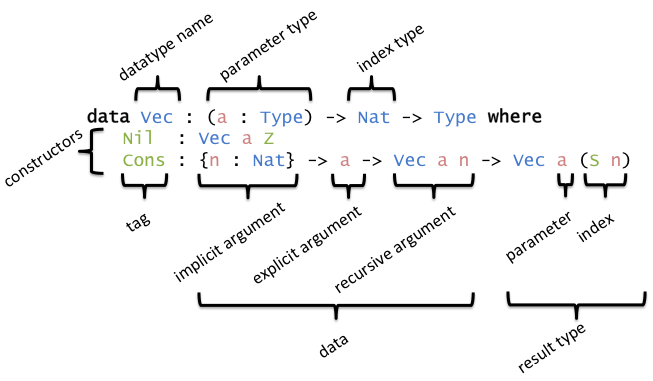
\includegraphics[scale=0.5]{Figures/AnatomyOfADatatype.png}
\end{center}
\caption{Annotated components of a datatype Declaration}
\label{fig:anatomydatatype}
\end{figure}

A datatype consists of a type constructor which lists what type-level arguments are required, and zero or more data constructors which describe how to create values of the datatype.
The type constructor has three components: a name for the datatype, types of any possible parameters, and the types of possible indices.
In Figure~\ref{fig:anatomydatatype} there is no syntactic difference between a parameter type or an index type since Idris figures that out automatically
\footnote{If an argument to a type constructor doesn't change in the data constructor declarations, Idris considers it a parameter, otherwise an index.},
unlike other dependently-typed languages like Agda which have a syntactic distinction.

Similarly to the type constructor, a data constructor needs a name, also called a \textit{tag}.
Following the tag, the data constructor declaration contains the types of the arguments stored in the constructor and the resulting type that must use the type constructor of the datatype.
In our example two constructors are declared, \ttconstructor{Nil} and \ttconstructor{Cons}.
The constructor \ttconstructor{Nil} doesn't hold any data, so it only needs to define the resulting type which is \tttype{Vec}~\ttvar{a}~\ttconstructor{Z} (a vector with length \ttliteral{0}).
The constructor \ttconstructor{Cons} contains three different types of arguments: an ordinary implicit argument, an ordinary explicit argument, and an explicit argument of the type itself (recursive); the resulting type for \ttconstructor{Cons} is \tttype{Vec}~\ttvar{a}~\texttt{(}\ttconstructor{S}~\ttvar{n}\texttt{)}, that is, a vector of length \ttliteral{1}\texttt{+}\ttvar{n} where \ttvar{n} is the length of the recursive argument.

\begin{asideblock}
  The colouring scheme for code presented in this paper uses the following conventions:
  \begin{quote}
  \begin{description}
    \item[\tttype{Blue}] is used for type constructors
    \item[\ttconstructor{Green}] is used for data constructors
    \item[\ttdec{Dark Red}] is used for top-level declarations
    \item[\ttvar{Light Red}] is used for locally-bound variables
    \item[\ttliteral{Purple}] is used for literals (integer, string, etc.)
    \item[\texttt{\textbf{Bold Black}}] is used for keywords (if, data, etc.)
  \end{description}
  \end{quote}

\end{asideblock}

\subsection{A description for datatypes}
\label{sub:ADescriptionforDatatypes}
It is now possible to try to represent a suitable datatype for descriptions.
Figure~\ref{fig:descriptiondatatype} presents one possible solution, influenced mainly by the work of \textcite{mcbride2010ornamental} and \textcite{diehl2014eliminators}.
Similarly based on that work, Section~\ref{sec:SynthesisingDescriptionstoTypes} will later present how to construct actual described types from these descriptions.

\begin{figure}[ht]
\begin{center}
    \includegraphics[scale=0.5]{Figures/ADescriptionforDatatypesSimple.png}
\end{center}
\caption{A datatype that describes other datatypes}
\label{fig:simpldescdatatype}
\end{figure}

The description datatype \tttype{Desc} has three main constructors:
\begin{itemize}
  \item  Constructor \ttconstructor{Ret} represents the end of a description
  \item  Constructor \ttconstructor{Arg} represents the addition of an argument of any type to a given description; the first argument of \ttconstructor{Arg} is the type of argument expected and the second argument is the rest of the description dependent on a value of that type.
  \item  Constructor \ttconstructor{Rec} represents a recursive argument of the described datatype. The argument of constructor \ttconstructor{Rec} is the specification of the rest of the description.
\end{itemize}

To get an idea on how descriptions for various interesting datatypes look like, the following paragraphs will show a series of examples providing a side-by-side comparison of ordinary declarations to descriptions.
The declaration of the trivial singleton type \tttype{Unit} is shown in Figure~\ref{fig:declunit}, and its corresponding description is shown in Figure~\ref{fig:descunit}.
Since the sole constructor \ttconstructor{MkUnit} doesn't contain any arguments, \ttconstructor{Ret} is used to simply end the description.

\begin{figure}[ht]
\begin{center}
  \subcaptionbox{Declaration of \tttype{Unit}\label{fig:declunit}}[.45\textwidth]{
    
\includegraphics[scale=0.5]{Figures/UnitDeclaration.png}
}
\subcaptionbox{Description of \tttype{Unit}\label{fig:descunit}}[.45\textwidth]{
    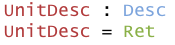
\includegraphics[scale=0.5]{Figures/UnitDescription.png}

}
\caption{The \tttype{Unit} datatype and its description}
\end{center}
\end{figure}

\paragraph{Constructor arguments}
A more interesting datatype is shown in Figure~\ref{fig:declpair}, namely the datatype \tttype{Pair} representing a pair of \tttype{Int} and \tttype{Bool}.
The translation to the corresponding description, as shown in Figure~\ref{fig:descpair}, seems straightforward. 
For each argument of \ttconstructor{MkPair} that is used \texttt{(}\ttvar{arg}~\texttt{:}~\ttvar{a}\texttt{)~->}~\ttvar{b}, the translation would be of the form \ttconstructor{Arg}~\ttvar{a}~\texttt{(\textbackslash}\ttvar{arg}~\texttt{=>}~\ttvar{b}\texttt{)}.
Finally, to specify the end of the description, \ttconstructor{Ret} is used.

\begin{figure}[ht]
\begin{center}
  \subcaptionbox{Declaration of \tttype{Pair}\label{fig:declpair}}[.45\textwidth]{
    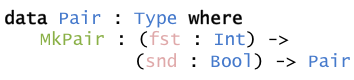
\includegraphics[scale=0.5]{Figures/PairDeclaration.png}
}
\subcaptionbox{Description of \tttype{Pair}\label{fig:descpair}}[.45\textwidth]{
    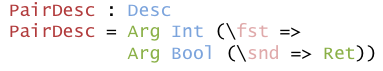
\includegraphics[scale=0.5]{Figures/PairDescription.png}

}
\caption{A pair of \tttype{Int} and \tttype{Bool}}
\end{center}
\end{figure}

A key aspect of algebraic datatypes is the ability to choose between multiple constructors.
Figure~\ref{fig:decleither} shows a simple datatype \tttype{Either} which provides two constructors \ttconstructor{Right} and \ttconstructor{Left}, than can hold a value of \tttype{Int} and \tttype{String} respectively.

\paragraph{Choice of constructors}
Since there is no explicit way to encode a choice between multiple constructor in the provided description, instead a boolean argument \ttvar{isRight} is used as a tag to determine which constructor is described.
If the value of \ttvar{isRight} is true then the resulting description is expected to be for the \ttconstructor{Right} constructor, otherwise
is is expected to be for the \ttconstructor{Left} constructor.
The description for each constructor is then specified in a similar fashion to datatypes with one constructor, such as \tttype{Pair} described above.

\begin{figure}[ht]
\begin{center}
  \subcaptionbox{Declaration of \tttype{Either}\label{fig:decleither}}[.45\textwidth]{
    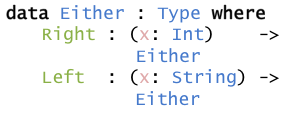
\includegraphics[scale=0.5]{Figures/EitherDeclaration.png}
}
\subcaptionbox{Description of \tttype{Either}\label{fig:desceither}}[.45\textwidth]{
    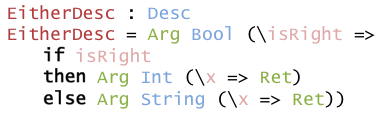
\includegraphics[scale=0.5]{Figures/EitherDescription.png}

}
\caption{the sum type of \tttype{Int} and \tttype{String}}
\end{center}
\end{figure}

\paragraph{Recursive arguments}
In addition to allowing the choice between multiple possible constructors, what makes algebraic datatypes interesting is the ability to
have recursive (or \textit{inductive}) instances. The simplest recursive datatype is the natural numbers \tttype{Nat} (shown in Figure~\ref{fig:declnat}) which has two constructors,
\ttconstructor{Zero} which represents \ttliteral{0} and the recursively defined \ttconstructor{Succ} which represents \ttliteral{1}+\ttvar{n} for any natural number \ttvar{n}.
The corresponding description is shown in Figure~\ref{fig:descnat} which is mainly built up using the principles introduced before.
The only addition is that the description for \ttconstructor{Succ} now uses \ttconstructor{Rec} to specify that it requires a recursive argument (to type \tttype{Nat} itself).

\begin{figure}[ht]
\begin{center}
  \subcaptionbox{Declaration of \tttype{Nat}\label{fig:declnat}}[.45\textwidth]{
    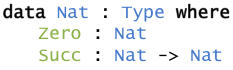
\includegraphics[scale=0.5]{Figures/NatDeclaration.png}
}
\subcaptionbox{Description of \tttype{Nat}\label{fig:descnat}}[.45\textwidth]{
    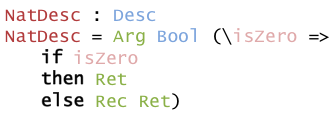
\includegraphics[scale=0.5]{Figures/NatDescription.png}

}
\caption{The Natural numbers (\tttype{Nat})}
\end{center}
\end{figure}

\paragraph{Parameters}
Figure~\ref{fig:decllist} shows one of the classical datatypes in functional programming languages, namely \tttype{List}.
Unlike \tttype{Pair} and \tttype{Either} which were monomorphic in the presented examples, \tttype{List} is polymorphic in its elements.
The way to represent parameters is by having them as arguments to the function describing the particular datatype, which allows them to be qualified over the whole description.
The description itself is built using the previously described methods and is shown in Figure~\ref{fig:desclist}. There is a Boolean argument \ttvar{isNil}, which encodes the choice between the two constructors of the list,
\ttconstructor{Nil} and \ttconstructor{Cons}.
Like the description for \ttconstructor{Zero}, the description for \ttconstructor{Nil} is simply \ttconstructor{Ret} since it doesn't accept any arguments.
The description for \ttconstructor{Cons} takes an argument of the parameter type (the head of the list), a recursive argument (the tail of the list) and then ends the description.

\begin{figure}[ht]
\begin{center}
  \subcaptionbox{Declaration of \tttype{List}\label{fig:decllist}}[.45\textwidth]{
    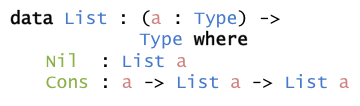
\includegraphics[scale=0.5]{Figures/ListDeclaration.png}
}
\subcaptionbox{Description of \tttype{List}\label{fig:desclist}}[.45\textwidth]{
    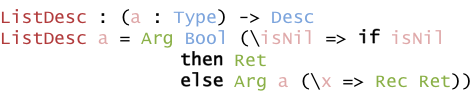
\includegraphics[scale=0.5]{Figures/ListDescription.png}

}
\caption{A polymorphic list of elements}
\end{center}
\end{figure}

The reader may have noticed that the datatypes presented so far are perfectly expressible in ordinary functional languages like Haskell or Standard ML\,\autocite{Milner:1997:DSM:549659}.
To really exploit the power of dependently-typed programming languages, it should be possible to express datatypes that may be indexed by values.
This will be discussed in Section~\ref{sub:Indexingdescriptions}.

\subsection{Indexing descriptions}
\label{sub:Indexingdescriptions}

To allow datatypes to be indexed by values, the description structure takes a parameter that describes what the type of indices must be.
Figure~\ref{fig:descriptiondatatype} shows an updated version of Figure~\ref{fig:simpldescdatatype}, that contains the necessary parameter \ttvar{ix} for indexing datatypes.
The constructors \ttconstructor{Ret} and \ttconstructor{Rec}, must also be updated to take a value of \ttvar{ix} in order to represent what the index of the result type and recursive argument must be respectively.
Descriptions that don't require indices can be converted to indexed descriptions by using the unit type \tttype{Unit} (or its syntactic form \tttype{()}) as index.

\begin{figure}[ht]
\begin{center}
    \includegraphics[scale=0.5]{Figures/ADescriptionforDatatypes.png}
\end{center}
\caption{Description for datatypes with possible indices}
\label{fig:descriptiondatatype}
\end{figure}

To give an example on how an indexed datatype looks like, let us take a new look at \tttype{Vec} from Figure~\ref{fig:anatomydatatype}.
Figure~\ref{fig:descvec} shows the corresponding description of \tttype{Vec} with comparable annotations.

\begin{figure}[ht]
\begin{center}
    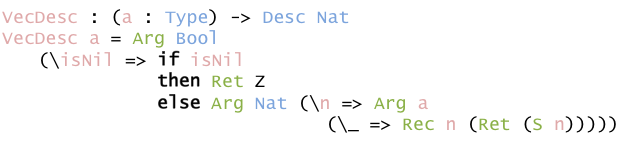
\includegraphics[scale=0.5]{Figures/VectorDescription.png}
\end{center}
\caption{Described version of \tttype{Vec}}
\label{fig:descvec}
\end{figure}


The type signature for the description of \tttype{Vec} mimics the one for the actual datatype closely, but there are nonetheless some differences.
There is now an explicit distinction between parameters and indices; the type for a parameter can still be specified as an argument for the description value,
whereas the type of an index must be provided to the \tttype{Desc} type constructor.
This is to ensure that all provided indices conform to the same expected type, while still allowing the values to change inside the description.

A Boolean argument \ttvar{isNil} is used to describe the choice between constructors \ttconstructor{Nil} and \ttconstructor{Cons}.
The constructor \ttconstructor{Nil} doesn't contain any data so we simply use \ttconstructor{Ret~Z}, which indicates that the description is finished and the resulting type is expected to have index \ttconstructor{Z}, analogously to Figure~\ref{fig:anatomydatatype}.
The constructor \ttconstructor{Cons} takes first two ordinary arguments: a \tttype{Nat} representing the length of the tail, i.e. the index of the recursive argument, and an argument of the parameter type \ttvar{a} representing the head.
Following these arguments we take a recursive argument representing the tail---specified using \ttconstructor{Rec}---that must have the value of the input \tttype{Nat} argument \ttvar{n} as index, i.e. the argument must be of type \tttype{Vec}~\ttvar{a~n}.
We finish the description with \ttconstructor{Ret} and specify that the resulting index must be \ttconstructor{S}~\ttvar{n}, just as in Figure~\ref{fig:anatomydatatype}.

\subsubsection{Challenges and limitations}
Even though it was possible to describe a variety of datatypes there are still a few questions that can be raised, such as: How is it possible to choose between more than two constructors? Why is there only one type for indices?
Why aren't the type of parameters required to be encoded inside the description datatype itself? How is it possible to represent more complex datatypes such as mutual recursive ones? I seek to answer these questions in the following paragraphs.

To encode the choice of more than two constructors, a simple solution could be to nest multiple Boolean values acting as a form of binary enumeration of tags.
However this encoding is fairly crude: it does not capture important information such as the names of constructors, requires a series of possibly complicated tests and is not easily extendible if one wants to extend descriptions
with new constructors. In Section~\ref{sub:AnInformativeEncodingofConstructors}, I will present a more sophisticated encoding that doesn't suffer from these limitations.

For more demanding datatypes that need more than one index, the indices must be uncurried using dependent pairs.
For example, a datatype with signature \texttt{(}\ttvar{n}~\texttt{:}~\tttype{Nat}\texttt{)~->~}\tttype{Fin}~\ttvar{n}~\texttt{->}~\tttype{Type} must use the dependent pair \tttype{(}\ttvar{n}~\texttt{:}~\tttype{Nat}~\tttype{**}~\tttype{Fin}~\ttvar{n}\tttype{)} as the type of its index.

Since parameters are usually quantified over the whole datatype (\textit{i.e.}, they do not change) it is possible to just accept them as external arguments when building
a description.
However, this encoding can preclude interesting generic programs from being written, such as the functorial map. In Chapter~\ref{cha:LevitatingIdris}, I will discuss a modification to the description datatype that permits encoding the types of
parameters directly.

Finally, there is the question on how more complicated datatypes are to be represented.
Datatypes that require recursive functions as arguments like \tttype{Desc}, can not currently be represented in the presented encoding and the description must be extended to be able to describe types as itself (see Section~\ref{sec:TheMostlyGentleArtofLevitation}).
Mutual recursive datatypes cannot be represented directly, but it is possible to use indices to represent an isomorphic representation.
For example, for two mutually recursive datatypes one could use a boolean argument as index which determines the actual datatype is currently described.
Unfortunately, a challenge that still persists is that the most complex inductive families---such as inductive-inductive and inductive-recursive definitions---can not be represented using the presented descriptions.

\subsection{An informative encoding of constructors}
\label{sub:AnInformativeEncodingofConstructors}
In Section~\ref{sub:ADescriptionforDatatypes} a Boolean variable was used to determine the choice between two constructors, and concluded that his approach had multiple disadvantages.
First of all, the Boolean encoding does not capture the names of the respective constructors which might be important when it is desired to pretty print or serialise a data structure.
Secondly, when there are more than two constructors, it can quickly become complicated to provide a suitable description.
Multiple Boolean arguments are required and mapping these Boolean values to description is not exactly straightforward.
For example, should two Boolean values encode the choice between 3 or 4 constructors?
Finally, and perhaps more importantly, it is not easy to modify the number of constructors easily with the Boolean encoding. That is, it might be desirable to compute a new description from a provided one and in that process to add a new constructor,
\textit{e.g.}, adding a default ``error'' constructor to each datatype.
This section presents a more informative encoding of constructors, and shows how it is possible to use that encoding when describing non-trivial datatypes.

To represent which constructors are available we first are going to declare two types (heavily inspired by \textcite{Dagand2013acosmology,diehl2014eliminators}) as shown in Figure~\ref{fig:ctorlabels}: \ttdec{CLabel} which represents a name for a constructor, and \ttdec{CEnum} which
represents a list of constructor names. For the sake of simplicity, the provided constructors in a \ttdec{CEnum} are assumed to be provided uniquely by the user, however one could stipulate such uniqueness condition explicitly if desired.
Figure~\ref{fig:vectctors} show an example of how to represent the available constructor names of \tttype{Vec}.


\begin{figure}[ht]
\begin{center}
  \subcaptionbox{Representation\label{fig:ctorlabels}}[.45\textwidth]{
    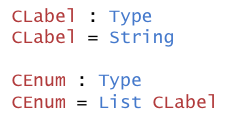
\includegraphics[scale=0.5]{Figures/AnInformativeEncodingofConstructorsLabels.png}
}
\subcaptionbox{Example: Constructors of Vec\label{fig:vectctors}}[.45\textwidth]{
    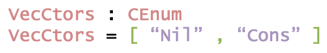
\includegraphics[scale=0.5]{Figures/VectorConstructors.png}

}
\caption{Constructor labels}
\end{center}
\end{figure}

Now that it is possible to represent the available constructors, we can encode a way of choosing a particular constructor tag. Figure~\ref{fig:ctortags} shows a datatype \tttype{Tag} with two constructors:
\ttconstructor{TZ} which represents the constructor that is on top of the current list and \ttconstructor{TS} which represents a constructor further along the list. As such, \tttype{Tag} specifies a valid index into a (non-empty) list of constructor tags.

This encoding has multiple advantages: it ensures that all constructor labels stored in our data exist in the expected list of constructors, it ensures that all datatypes which are dependent on a tag must have at least one constructor, and as a consequence
it is possible to specify the empty type by simply requiring a tag on an empty list of expected constructors (since such value would be impossible to create).
This encoding makes it possible to use tactics in Idris to automate the retrieval of a tag given a constructor label; something which saves time when constructing
values manually.

\begin{figure}[ht]
\begin{center}
    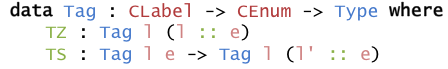
\includegraphics[scale=0.5]{Figures/AnInformativeEncodingofConstructorsTags.png}
\end{center}
\caption{Tags: A Structure for Picking a Constructor from a Label Collection}
\label{fig:ctortags}
\end{figure}

For the constructors of \tttype{Vec}, Figure~\ref{fig:vecctor} shows an example on what the tag values are. For \ttconstructor{Nil} the value is \ttconstructor{TZ} since it is the first in the list of \ttdec{VecCtors}, and for \ttconstructor{Cons} the value
is \ttconstructor{TS~TZ} since it is the second. Since there are only two elements in \ttdec{VecCtors}, it shouldn't be possible to create any other valid constructor tag, and as therefore it is a good representative for enumerating the constructors of \tttype{Vec}.

\begin{figure}[ht]
\begin{center}
  \subcaptionbox{Tag for \ttconstructor{Nil}\label{fig:vecctornil}}[.45\textwidth]{
    
\includegraphics[scale=0.5]{Figures/VectorNilTag.png}
}
\subcaptionbox{Tag for \ttconstructor{Cons}\label{fig:vecctorcons}}[.45\textwidth]{
    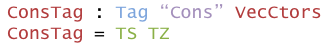
\includegraphics[scale=0.5]{Figures/VectorConsTag.png}

}
\caption{Example: Tags for constructors of \tttype{Vec}}
\label{fig:vecctor}
\end{center}
\end{figure}


\subsection{A constructive type of choice}
\label{sub:AConstructiveTypeofChoice}
Similarly to how \texttt{\textbf{if}} was used to map \tttype{Bool} values to the descriptions of the various constructors of a datatype in Section~\ref{sub:ADescriptionforDatatypes}, it is desirable to have a way
to map \tttype{Tag} values to suitable values of a desired type.  The following section will describe the \ttdec{switch} function that does exactly this.

Since the count of constructors for a datatype can vary in size, it is necessary to calculate a type that allows mapping the tag of each constructor to a suitable value (shown in Figure~\ref{fig:smallpiop}). 
It is essentially a function that provides a one-to-one mapping from the list of constructors to a series of right-nested pairs ending with \tttype{()}.
The type of the resulting value \ttvar{prop} can be dependent on the input constructor tag, and therefore the function is called $\pi$ or the \textit{small pi operator}.
The operator $\pi$ is small in the sense that unlike the dependent function type $\Pi$ which allows the result to dependent on any type of input, $\pi$ only allows dependencies on constructor tags.

\begin{figure}[ht]
\begin{center}
    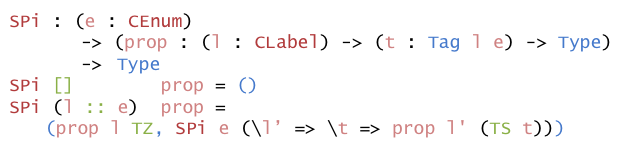
\includegraphics[scale=0.5]{Figures/AConstructiveTypeofChoice.png}
\end{center}
\caption{The small pi operator: type for case analysis based on constructor tags}
\label{fig:smallpiop}
\end{figure}

Given a way to map a list of constructors to a list of values using $\pi$, it is now possible to define \ttdec{switch} which can look up the corresponding result value in the map for a particular \tttype{Tag}.
The function \ttdec{switch} is shown in Figure~\ref{fig:switchctor} and has two branches: if the constructor to map is the first one in a list of constructors, it simply returns the first value in the corresponding mapping, otherwise
it continues the search using the rest of the provided elements (skipping the first constructor and its corresponding mapping).
Since there can be no value of \tttype{Tag} on an empty enumeration of constructors, it is not required to handle that case.

\begin{figure}[ht]
\begin{center}
    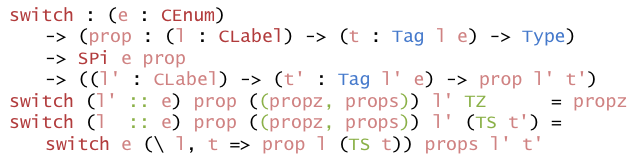
\includegraphics[scale=0.5]{Figures/AConstructiveChoice.png}
\end{center}
\caption{Calculation of a property based on a specific constructor tag}
\label{fig:switchctor}
\end{figure}

As an example, Figure~\ref{fig:vecdescim} shows the description of \tttype{Vec} (from Figure~\ref{fig:descvec}) again, but this time using the new constructor tag encoding instead of a Boolean variable.

\begin{figure}[H]
\begin{center}
    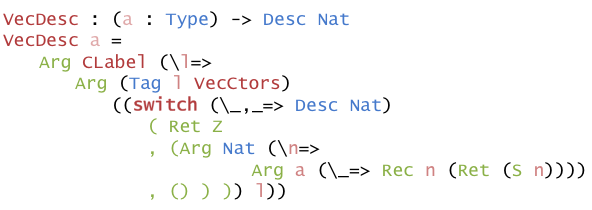
\includegraphics[scale=0.5]{Figures/VectorDescriptionImproved.png}
\end{center}
\caption{Description of Vec given a Constructor Tag}
\label{fig:vecdescim}
\end{figure}

In summary, while the description might initially seem more complicated than before, it has a couple of clear advantages: the encoding now contain the constructor tag and it is possible to choose between more than two constructors at the same time.

\section{Synthesising types from descriptions}
\label{sec:SynthesisingDescriptionstoTypes}
In Section~\ref{sec:TheGenericStructureofInductiveDataTypes} I had shown how it was possible to create descriptions that support many common datatypes in Idris.
In this section I will present a way to convert or \textit{synthesise} these descriptions to actual types, that allows the programmer to construct values of these described types with actual data.

\subsection{Datatype synthesis}
\label{sub:DatatypeSynthesis}
It is finally time to convert the description to an actual type. Figure~\ref{fig:synthdata} shows the \ttdec{Synthesise} function which takes a description, the final form of that datatype and the resulting index, then it returns a type which can contain the described data.

\begin{itemize}
  \item If we reach the end of the description \textit{i.e.}, \ttconstructor{Ret}, the only thing that we need to ensure is that the provided resulting index matches the expected index provided in the description. In order to apply such constraint we use the propositional equality type.
  \item For recursive arguments \textit{i.e.}, \ttconstructor{Rec}, we construct a dependent pair where the first argument contains a value of the fully-synthesised type with the given index and the second argument contains the synthesised version of the rest of the provided description. The reason that we need the final form of the datatype in order to construct a recursive argument is due to the fact that if we call \ttdec{Synthesise} recursively on that argument we would get stuck in an infinite loop!
  \item For ordinary arguments \textit{i.e.}, \ttconstructor{Arg}, we also create a dependent pair. The first argument of the dependent pair is a value \ttvar{arg} of the provided type \ttvar{a}, and the second argument is the synthesis of the rest of the provided description \ttvar{d} given \ttvar{arg}. This is isomorphic to how an ordinary constructor would store the data and as such the dependent pair serves a good target structure for our synthesis.
\end{itemize}
Since the dependent pair is used as the target type for the synthesis, it itself must be a core part of the type theory similarly to the propositional equality, if we want to treat all datatype declarations as describable.

\begin{figure}[ht]
\begin{center}
    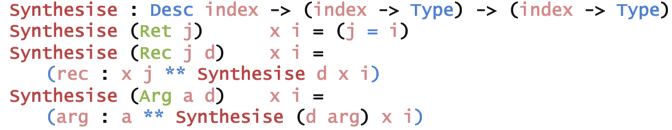
\includegraphics[scale=0.5]{Figures/SynthesisingData.png}
\end{center}
\caption{Synthesising Descriptions into Actual Types}
\label{fig:synthdata}
\end{figure}

We are able to actual types using \ttdec{Synthesise} from the provided descriptions.
However, a problem occurs when we want to use \ttdec{Synthesise} since it requires the final form of the described datatype as input but the only way to synthesise the datatype is using \ttdec{Synthesise} itself.
In order to ``tie the knot'' and complete input for \ttdec{Synthesise}, we define a datatype \tttype{Data} that takes a description and provides the final form of the described datatype (see Figure~\ref{fig:datafromdesc}).
\tttype{Data} has only one constructor namely \ttconstructor{Con} which takes as input the synthesised version of the description \ttvar{d} with \tttype{Data}~\ttvar{d} serving as argument for the final form of the datatype in \ttdec{Synthesise}. This works since each time we face a recursive argument it must be constructed using \ttconstructor{Con} which avoids an infinite loop in \ttdec{Synthesise} as long as the elements that are constructed are smaller in size.

\begin{figure}[ht]
\begin{center}
    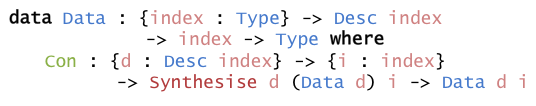
\includegraphics[scale=0.5]{Figures/TyingTheSynthesisKnot.png}
\end{center}
\caption{Knot-tying the Synthesised Description with Itself}
\label{fig:datafromdesc}
\end{figure}

\subsection{Example: Constructing vectors}
\label{sub:Example:Constructing Vectors}

To get a more concrete intuition on how it is possible to construct data values of described types, this section will look at the synthesised version of \tttype{Vec}.
Figure~\ref{fig:synthversvecdesc} shows \ttdec{Vec} which is a function mimicking its corresponding type constructor, and it even shares the same type signature.
The function \ttdec{Vec} returns a described type using \tttype{Desc} passing along the description of \tttype{Vec} and its required parameters (\textit{i.e.}, \ttdec{VecDesc}~\ttvar{a}), 
and additionally the expected value of the result index (\textit{i.e.}, \ttvar{n}).

\begin{figure}[ht]
\begin{center}
    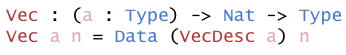
\includegraphics[scale=0.5]{Figures/VectorSynthesisedDesc.png}
\end{center}
\caption{Synthesised Version of Vector Description}
\label{fig:synthversvecdesc}
\end{figure}

A simple example representing the vector \ttconstructor{[}\ttliteral{1}~\ttconstructor{,}~\ttliteral{2}~\ttconstructor{,}~\ttliteral{3}\ttconstructor{]} is presented in Figure~\ref{fig:exmvecsynthvecdesc}. Although the value might seem a bit overwhelming at first, it follows a simple pattern:
each time a value of \ttdec{Vec} is needed \ttconstructor{Con} is used, followed by its required arguments in the form of nested dependent pairs, and finally with \ttconstructor{Refl}, which ensures
that the provided index of the value matches up with the expected one.
There are 4 occurrences of \ttconstructor{Con} and \ttconstructor{Refl} in the example, three for  \ttconstructor{Cons} and one for \ttconstructor{Nil}.
For all cases the first two arguments represent the constructor label and associated tag. 
For \ttconstructor{Cons}, the first following argument is the length of the rest of the vector (the value of index \ttvar{n}) followed by the value of the list head and the list tail, ending with \ttconstructor{Refl}.
For \ttconstructor{Nil}, the value is ended with \ttconstructor{Refl} since it doesn't contain any data.


\begin{figure}[ht]
\begin{center}
    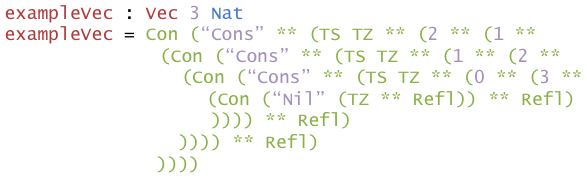
\includegraphics[scale=0.5]{Figures/VectorSynthesisedExample.png}
\end{center}
\caption{Example vector representing \ttconstructor{[}\ttliteral{1}~\ttconstructor{,}~\ttliteral{2}~\ttconstructor{,}~\ttliteral{3}\ttconstructor{]} as a value of a synthesised description}
\label{fig:exmvecsynthvecdesc}
\end{figure}

As might have become apparent there are a couple of shortcomings in the example, or rather the way values of described types are constructed.
One shortcoming is that there is a lot of boilerplate required when values are constructed, which makes the result somewhat unreadable.
A solution to overcome that shortcoming is presented in the next paragraph. Another shortcoming is that the resulting terms become very large, and in turn slowing down program execution, compared to the original
version of the datatype. For example, \ttconstructor{Nil} becomes inflated to \ttconstructor{Con~(}\ttliteral{"Nil"}~\ttconstructor{** (TZ ** Refl))} which is significantly more complex. A description on how to improve the size of resulting terms and
speed up the performance of dependent programs is presented in Chapter~\ref{cha:OptimizingIdrisforFlight}.

In order to make creation of values of described types easier and the resulting terms more readable, it is possible to use functions as synonyms for the constructors.
Figure~\ref{fig:funcconstrsynthvec} shows \ttdec{Nil} and \ttdec{Cons} as synonyms for the described version of \ttconstructor{Nil} and \ttconstructor{Cons} respectively.
Since Idris can infer the values of \ttvar{a} and \ttvar{n} automatically in this context, they are converted to implicit parameters in these synonyms (which further increases readability).

\begin{figure}[ht]
\begin{center}
    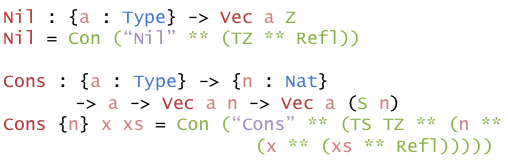
\includegraphics[scale=0.5]{Figures/VectorSynthesisedConstructors.png}
\end{center}
\caption{Functions for constructing values of synthesised vector description}
\label{fig:funcconstrsynthvec}
\end{figure}

Using these synonyms, the constructor of the value in example in Figure~\ref{fig:exmvecsynthvecdesc} becomes simpler and much more readable. Figure~\ref{fig:exmvecsynthvecdescconstrs} shows the updated version,
and it looks almost exactly like the original value it needed to describe \ttconstructor{[}\ttliteral{1}~\ttconstructor{,}~\ttliteral{2}~\ttconstructor{,}~\ttliteral{3}\ttconstructor{]}.


\begin{figure}[ht]
\begin{center}
    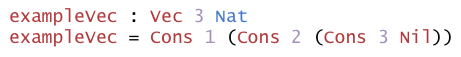
\includegraphics[scale=0.5]{Figures/VectorSynthesisedConstructorsExample.png}
\end{center}
\caption{More readable version of \ttconstructor{[}\ttliteral{1}~\ttconstructor{,}~\ttliteral{2}~\ttconstructor{,}~\ttliteral{3}\ttconstructor{]} using aliases from Figure~\ref{fig:funcconstrsynthvec}}
\label{fig:exmvecsynthvecdescconstrs}
\end{figure}

\section{The (mostly) gentle art of levitation}
\label{sec:TheMostlyGentleArtofLevitation}
The previous sections presented a series of constructions that makes it possible to have described types.
What may have become apparent for the reader is that many of these constructions such as \tttype{Data}, \tttype{Tag} and \ttdec{switch} cannot themselves be described,
since they are necessary building blocks for having descriptions.
However, what might be surprising is that the description type \tttype{Desc} itself, isn't in fact limited by such a constraint
and can be described using itself.
This is the key point addressed by \textcite{Chapman:2010:GAL:1863543.1863547} in "The Gentle Art of Levitation".

The description datatype \tttype{Desc} contains many of the constructors needed to describe itself.
However, one might experience trouble when trying to describe \ttconstructor{Arg} since it requires an argument of the following type:
\texttt{(}\ttvar{a}~->\tttype{Desc}~\ttvar{ix}\texttt{)}.
This argument describes a function which result type is the datatype itself (a so-called higher-order inductive argument), which \ttconstructor{Rec} isn't strong enough to express since it only permits primitive recurrences.
Figure~\ref{fig:deschrec} shows a new constructor \ttconstructor{HRec}, which allows specification of such higher-order inductive arguments, it takes a type \ttvar{a} which specifies
the expected input type of such argument in addition to the rest of arguments that are expected by \ttconstructor{Rec}.

\begin{figure}[ht]
\begin{center}
    
\includegraphics[scale=0.5]{Figures/ADescriptionForDatatypesExtended.png}
\end{center}
\caption{A constructor for \tttype{Desc} to represent higher-order recursion}
\label{fig:deschrec}
\end{figure}

The function \ttdec{Synthesise} must be extended with a clause for \ttconstructor{HRec}. Figure~\ref{fig:synthhrec} shows the corresponding clause,
which looks very similar to the one for \ttconstructor{Rec}, except the first component now requires a function from the provided type \ttvar{a} to the datatype itself instead of just a reference
to the datatype.

\begin{figure}[ht]
\begin{center}
    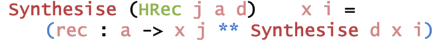
\includegraphics[scale=0.5]{Figures/SynthesisingDataExtended.png}
\end{center}
\caption{Synthesising \ttconstructor{HRec} to a real type}
\label{fig:synthhrec}
\end{figure}

Finally, all the required constructors are present and it is now possible to piece together a description for \tttype{Desc}. Figure~\ref{fig:descdesc} shows the complete description, including for the newly added
\ttconstructor{HRec} constructor. The description of \tttype{Desc} is parametrised by the type of indices \ttvar{ix} that possible derived descriptions can have, and is not indexed by anything particularly interesting (the unit type \tttype{()} is used in the figure).
The description for each constructor is translated using the same techniques presented in Section~\ref{sec:TheGenericStructureofInductiveDataTypes}. The only interesting case is the one for \ttconstructor{Arg}, which uses \ttconstructor{HRec ()}~\ttvar{a}~\texttt{(}\ttconstructor{Ret ()}\texttt{)} to represent the higher-order inductive argument \texttt{(}\ttvar{a}~->~\tttype{Desc}~\ttvar{ix}\texttt{)}.

\begin{figure}[ht]
\begin{center}
    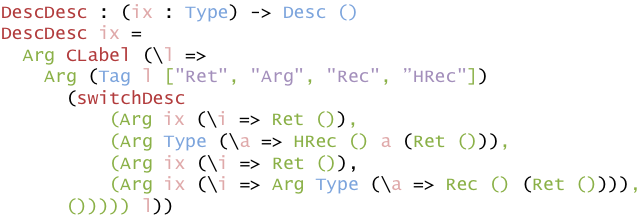
\includegraphics[scale=0.5]{Figures/DescriptionDescription.png}
\end{center}
\caption{Describing the \tttype{Desc} datatype itself}
\label{fig:descdesc}
\end{figure}

Perhaps, the key thing to notice is that a function \ttdec{switchDesc} was used instead of \ttdec{switch} when describing \tttype{Desc}.
Figure~\ref{fig:switchdesc} shows how \ttdec{switchDesc} is defined by specialising \ttdec{switch}. However, if \tttype{Desc} is a described type based on \ttdec{DescDesc} then such a definition would be circular.
This is because the general \ttdec{switch} requires the result type \tttype{Desc} to be given as an argument, but \tttype{Desc} is dependent on \ttdec{DescDesc}. Therefore, \textcite{Chapman:2010:GAL:1863543.1863547} define \ttdec{switchDesc} to be handled specially in their type theory, eliding the definition of the body
and hard-wiring its return type to be \tttype{Desc}
\footnote{Of course, such trick only works if the type \tttype{Desc} is already known to be in the meta-theory.
However, the knowledge of its elements is not necessarily required and it is possible to inspect these in a similar fashion to other datatypes.}.
Now, \ttdec{DescDesc} can be type checked without any issues and \textit{levitation} is achieved.

\begin{figure}[H]
\begin{center}
    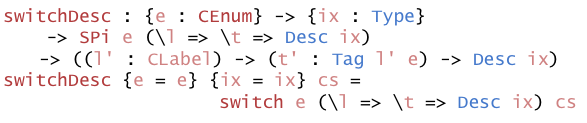
\includegraphics[scale=0.5]{Figures/AConstructiveChoiceDesc.png}
\end{center}
\caption{A specialised version of \ttdec{switch} which returns descriptions}
\label{fig:switchdesc}
\end{figure}

\section{Ensuring tagging of descriptions}
\label{sec:Ensuring tagging of descriptions}
The plain description type \tttype{Desc} accepts descriptions of any form, which can limit how some algorithms are written.
For example, it might be useful to pretty print the constructor tags different from data elements, and therefore it would be nice if the type system ensured
that it was possible to know where the tags were.
Similarly, if one needs to extend the number of constructors in a described type, it is necessary to know how the tagging is made.

\begin{figure}[ht]
\begin{center}
    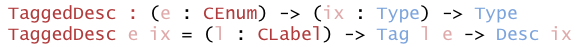
\includegraphics[scale=0.5]{Figures/TaggingDescriptions.png}
\end{center}
\caption{A datatype for representing descriptions with tags}
\label{fig:tagdesc}
\end{figure}

\textcite{Dagand2013acosmology} suggests that it is possible to create a type representing tagged descriptions while keeping
the same level of expression (see Figure~\ref{fig:tagdesc} for an inspired implementation).
The type \ttdec{TaggedDesc} represents the type of functions from tags to descriptions, which is exactly the same as what the function \ttdec{switchDesc} returns.

\begin{figure}[ht]
\begin{center}
    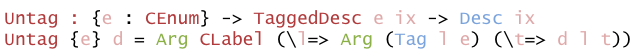
\includegraphics[scale=0.5]{Figures/DetaggingDescriptions.png}
\end{center}
\caption{Converting tagged descriptions to ordinary descriptions}
\label{fig:untagdesc}
\end{figure}

A function \ttdec{Untag} which converts tagged descriptions to ordinary descriptions is shown in Figure~\ref{fig:untagdesc}.
The \ttdec{Untag} function converts the function arguments of \tttype{TaggedDesc} to data arguments by using the \ttconstructor{Arg}, which ensures
that the provided tags are stored with the rest of the data arguments when constructed.

A key advantage of accepting a \ttdec{TaggedDesc} and then calling \ttdec{Untag}---instead of merely accepting an ordinary \tttype{Desc}---is that the type system
gains knowledge that the first two arguments of data are of type \ttdec{CLabel} and \tttype{Tag}.
This permits the algorithm designer, to treat those arguments differently when \textit{e.g.}, pretty printing the datatype.

\begin{figure}[ht]
\begin{center}
    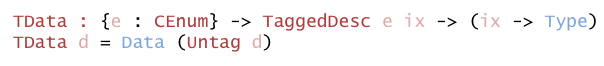
\includegraphics[scale=0.5]{Figures/TaggedDescriptionData.png}
\end{center}
\caption{The described version of tagged descriptions}
\label{fig:tagdata}
\end{figure}

Figure~\ref{fig:tagdata} shows a type \ttdec{TData} which is the analogous of \tttype{Data} for tagged descriptions.
The definition is simple as it simply converts the provided tagged description to an ordinary description, and then calls \tttype{Data} on that.
Therefore, the main point of using \ttdec{TData} is to ease the conversion between tagged descriptions and dependent described types.



\chapter{Partial evaluation}
\label{cha:PartialEvaluation}

The description datatype \tttype{Desc} presented in Chapter~\ref{cha:GenericProgramming} was very flexible and could express many common algebraic datatypes.
However as discussed in Section~\ref{sub:Example:Constructing Vectors}, the corresponding terms used to construct values of described types were much larger and more complex than the corresponding values of ordinary datatypes, yet they do not convey much more relevant information.
The reason is that much of the contained data is static information needed solely to provide the right form for generic algorithms, but is not needed when dealing with specific structures.
Therefore this chapter discusses relevant partial evaluation techniques needed to minimise the size of the large terms in order to improve runtime performance, by specialising the algorithm with regards to relevant static data when possible.

\section{The static nature of programs}
\label{sec:Thestaticnatureofprograms}
It hardly comes as a surprise, that for many programs, not all of their input might be dynamic.
Sometimes it is due to the way programs are structured in a modular fashion (e.g. functions or objects), where readability and reusability are highly valued even if some of the input to these structures is static.
For example, writing \ttdec{minutesInADay}~\texttt{=}~\ttliteral{24}~\texttt{*}~\ttliteral{60} is usually seen as more preferable to writing \ttdec{minutesInADay}~\texttt{=}~\ttliteral{1440}, since
it better captures the intent of the programmer.
Other times, it may be because that the input is known ahead of time and therefore in some way hard-coded (\textit{e.g.}, configuration files or constants).
No matter what reason, it can be said that any program \ttdec{p} accepts a series of static input \ttvar{i$_{s_0}$}\texttt{\ldots}\ttvar{i$_{s_n}$}~\texttt{$\in$}~\ttvar{I$_{s}$} and a series of dynamic input \ttvar{i$_{d_0}$}\texttt{\ldots}\ttvar{i$_{d_m}$}~\texttt{$\in$}~\ttvar{I$_{d}$}, resulting in some output \ttvar{O}.
%A program can be said to have both static and dynamic input

In many cases it is desirable to only compute programs with known input once and for all, instead of suffering a performance loss every time the program is run.
One technique for static computation of programs, is called \textit{partial evaluation}\,\autocite{Jones:1993:PEA:153676}. A program that does partial evaluation \ttdec{mix} is called a \textit{partial evaluator}, and accepts as input another program (often called the \textit{object program}) and a series of static input for that particular program.
The result of \ttdec{mix} is a new program called the \textit{residual program} which is \textit{specialised} with regards to the specified static input.
That is for any program \ttvar{p}, partially evaluating it regarding its static input \ttvar{I$_s$}---that is \ttdec{mix}~\ttvar{p}~\ttvar{I$_s$}---results in a residual program \ttvar{p$_r$}.
The residual program \ttvar{p$_r$} accepts the remaining dynamic input \ttvar{I$_d$} and produces the same expected result \ttvar{O}; therefore, the following equation is satisfied: \ttvar{p}~\ttvar{I$_s$}~\ttvar{I$_d$}~\texttt{$\equiv$}~\texttt{(}\ttdec{mix}~\ttvar{p}~\ttvar{I$_s$}\texttt{)}~\ttvar{I$_d$}~\texttt{$\equiv$}~\ttvar{p$_r$}~\ttvar{I$_d$}~\texttt{$\equiv$}~\ttvar{O}.

The canonical example of partial evaluation \autocite{Jones:1993:PEA:153676,mogensen1997,taha2004gentle} is the \ttdec{power} function which calculates $x^n$ and is shown in Figure~\ref{fig:powexmp}.
In this version of \ttdec{power}, the control flow is mostly determined by its first variable \ttvar{n}.
Therefore, if \ttvar{n} is provided statically then it is possible to specialise \ttdec{power} to avoid the branching dependent on \ttvar{n} and recursion at run-time.

\begin{figure}[ht]
\begin{center}
    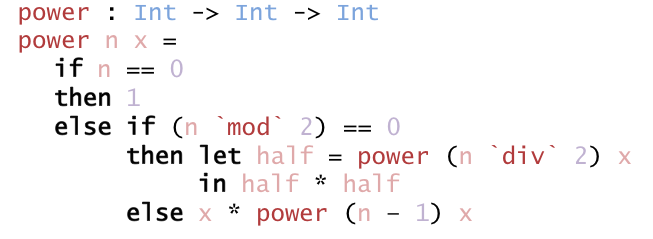
\includegraphics[scale=0.5]{Figures/PowerExample.png}
\end{center}
\caption{The function \ttdec{power} which calculates the value $x^n$ for input integers $x$ and $n$}
\label{fig:powexmp}
\end{figure}

Figure~\ref{fig:powspec} shows a partially evaluated version of power, where \ttvar{n} is fixed statically to \ttliteral{5}.
To achieve such optimisation, the partial evaluator must support various interesting optimisation techniques such as \textit{constant folding}, \textit{program point specialisation} and \textit{unfolding}/\textit{transition compression} \autocite{Jones:1993:PEA:153676} which will be discussed further in Section~\ref{sec:Anoptimisingpartialevaluator}.

\begin{figure}[ht]
\begin{center}
    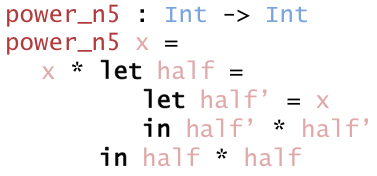
\includegraphics[scale=0.5]{Figures/PowerSpecialised.png}
\end{center}
\caption{\ttdec{power} specialised with regards to \ttvar{n} set to \ttliteral{5}}
\label{fig:powspec}
\end{figure}

\section{An optimising partial evaluator}
\label{sec:Anoptimisingpartialevaluator}
Since the only requirement for a partial evaluator is that the residual program depends only on some dynamic input, it is simple to make a trivial partial evaluator.
The trivial partial evaluator simply ``hard-codes'' the provided static input, and otherwise leaves the input object program unchanged.
However, such partial evaluator is hardly interesting from a performance perspective.
In order for a partial evaluator to be interesting, it must be able to utilise a set of optimisation techniques while evaluating a program.
In this section, three commonly used optimisation techniques for partial evaluators are presented: constant folding, program point specialisation and unfolding.

\subsection{Program Point Specialisation}
\label{sub:Program Point Specialisation}
According to \textcite{Jones:1993:PEA:153676}, a \textit{program point} is a referable point of execution that forms a part of a larger program.
For many modern languages, a program point would be a function or procedure; however, it could also be a label in an assembly language or a clause definition in a logic language.
Program point specialisation is the act of creating new versions of existing program points specialised with regards to some statically provided input.
That is, a specialised version of a program point \ttvar{l} is a pair \texttt{$\langle$}\ttvar{l}~\texttt{,}~\ttvar{I$_s$}\texttt{$\rangle$} such that \ttvar{I$_s$} is some provided
static input somewhere in the program.
Figure~\ref{fig:powxuf} shows a version of \ttdec{power} where \ttvar{n} is specialised to \ttliteral{5}, and all recursive calls to power are partially evaluated using program point specialisation.

\subsubsection{Polyvariant Specialisation}
\label{par:PolyvariantSpecialisation}
A program point specialisation is said to be \textit{polyvariant} if there are multiple versions of originally the same program point specialised with varying static input \autocite{Hughes:1999:LNCS:1706,Jones:1993:PEA:153676}.
For example, the \ttdec{power} function is specialised with regards to different values for the exponent \ttvar{n} in Figure~\ref{fig:powxuf} and is therefore polyvariant.

A special case of polyvariant specialisation, is when a program point specialisation is said to exhibit a \textit{polyvariant division}. A division is polyvariant if the set of static arguments varies for specialised versions of that particular program point.
Finding a division between static and dynamic arguments of a program point is not a trivial task, and especially not finding a polyvariant one.
Section~\ref{sec:Binding-timeAnalysisofPrograms} discusses what techniques there are for finding such divisions.


\subsection{Constant folding}
\label{sub:Constant folding}
Simply put, constant folding is the idea of reducing pure expressions with statically known arguments as much as possible.
This includes simple primitive arithmetic and logic operations such as addition, multiplication, conjunction and equality testing; but also pruning statically-determined branching such as \texttt{\textbf{if}}-expressions\,\autocite{Wegman:1991:CPC:103135.103136,Jones:1993:PEA:153676} or \texttt{\textbf{case}}-trees\,\autocite{boquist1999code}.

\paragraph{Reducing arithmetic and logical operations}
\label{par:Reducingarithmeticandlogicaloperations}
If all the operands of a given arithmetic or logical operator are statically determined then reducing such an operation is simply evaluating the result, \textit{e.g.}, for an expression \ttliteral{2}~\texttt{+}~\ttliteral{2} it can simply be reduced to the value \ttliteral{4}.
However, constant propagation algorithms are often allowed to do other types of simplifying reductions where some operands are dynamic, such as reducing addition with \ttliteral{0}, multiplication with \ttliteral{1} or conjunction with \ttconstructor{True}.

Figure~\ref{fig:powxcf} shows \ttdec{power} from Figure~\ref{fig:powexmp} again under specialisation with \ttvar{n} set to \ttliteral{5}. In the figure, all arithmetic expressions (namely \ttdec{mod}, \ttdec{div} and ``\texttt{-}'') and logic expressions (namely ``\texttt{==}'') have been reduced to simple integer values.

\begin{figure}[ht]
\begin{center}
    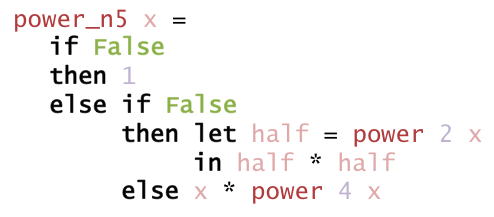
\includegraphics[scale=0.5]{Figures/PowerExampleConstantFolding.png}
\end{center}
\caption{Reduction of arithmetic and logical expression in \ttdec{power} with \ttvar{n} set to \ttliteral{5}}
\label{fig:powxcf}
\end{figure}


\paragraph{Branch pruning}
\label{par:Branch pruning}
If a conditional is somehow reduced to a constant value by another optimisation, it is possible to completely eliminate branching in \texttt{\textbf{if}}- or \texttt{\textbf{case}}-expressions.
For \texttt{\textbf{if}}-expressions, if the conditional is reduced to \ttconstructor{True} then the whole expression is reduced to the \texttt{\textbf{then}} branch, otherwise (if it is reduced to \ttconstructor{False}) then the whole expression is reduced to the \texttt{\textbf{else}} branch.
For \texttt{\textbf{case}}-expressions, they are simply reduced to the branch that matches the pattern of the value provided.

Figure~\ref{fig:powxbp} shows an updated version of \ttdec{power\_n5} from Figure~\ref{fig:powxcf}.
Since all \texttt{\textbf{if}}-expressions depended on constant values, it was possible to completely eliminate branching from the result.

\begin{figure}[ht]
\begin{center}
    
\includegraphics[scale=0.5]{Figures/PowerExampleBranchPruning.png}
\end{center}
\caption{Pruning of statically determined branches for \ttdec{power\_n5}}
\label{fig:powxbp}
\end{figure}

Using more advanced optimisation techniques, it is still possible to reduce branches of \texttt{\textbf{case}}-expressions if only some parts of the conditional are statically determined. If the reader is interested, please refer to \textcite{PeytonJones:1992:IFL:129390} and \textcite{boquist1999code}.

\subsection{Unfolding}
\label{sub:Unfolding}
To avoid too many unnecessary indirections in specialised programs, a perhaps important technique is unfolding.
Unfolding is usually done at sites where there are function calls and corresponds to inlining the body of the function that is called at the place where it is called.
In addition to simply inlining the body of the function, unfolding usually needs to do renaming of local variables to avoid clashes with the external environment.
For a languages with labels, transition compression serves as a good analogue to unfolding, where a jump to a label is replaced with the following instructions.
While there are many advantages to unfolding, and likewise transition compression, if not careful the partial evaluator can end up in an infinite loop or the resulting code can end up with exponential size in the case of poorly chosen static variables\,\autocite{Jones:1993:PEA:153676}.
Therefore, unfolding cannot be seen as a generally safe technique and must be used with care in places where there are branching or similar.

\begin{figure}[ht]
\begin{center}
    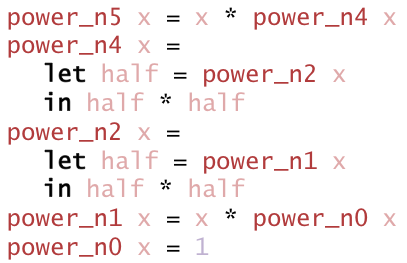
\includegraphics[scale=0.5]{Figures/PowerExampleBranchUnfolding1.png}
\end{center}
\caption{The function \ttdec{power\_n5} and necessary dependencies after program point optimisation
and constant folding}
\label{fig:powxuf}
\end{figure}

Figure~\ref{fig:powxuf} shows further transformation of the code in Figure~\ref{fig:powxbp}, after the completion of necessary program point specialisation and constant folding.
As can be observed in the figure, there is alot of indirection in each specialisation of \ttdec{power} requiring a new function call for all cases except when \ttvar{n} is set to \ttliteral{0}.
It is therefore desirable to do unfolding to improve performance, and doing unfolding for \ttdec{power\_n5} brings us back to Figure~\ref{fig:powspec} which is the final form of the optimisation.


\section{Dividing the static and dynamic parts of a program}
\label{sec:Binding-timeAnalysisofPrograms}
In Section~\ref{sec:Thestaticnatureofprograms}, an argument was made that programs usually contain both static and dynamic input.
A division for a program point is specifically an assignment of a binding-time, either static or dynamic, to each argument and expression at that point.
There are generally two non-exclusive ways to get the binding-time of variables, one is using a binding-time \textit{analysis}
and the other is requiring \textit{annotation} of binding-time by the user using \textit{e.g.}, \textit{two-level} syntax\,\autocite{Nielson:1989:TSA:75491.75492,Jones:1993:PEA:153676}.
In the broadest sense, binding-time analysis is vaguely similar to type inference while checking whether binding-time is well-annotated is vaguely similar to type checking.

\subsection{Binding-time analysis}
\label{sub:Binding-time analysis}
The core idea in a binding-time analysis (BTA) is to infer from given initial program input, what parts of a program may be executed statically.
For functional programming languages like Idris, there are roughly four classes of expressions which have different set of binding-time behaviour:
constants, variables, function application/operators, and conditionals/case analysis.
\begin{itemize}
  \item Constants are always assumed to be static, independent of whether they are for primitive types such as integers or strings, or base constructors of datatypes.
  \item The binding time for a variable usually depends on the type of variable and the surrounding environment.
    If the variable is let-bound or globally declared it will get the binding-time of the expression that is assigned to it.
    For function arguments they are assumed to be static in the function body, unless they appear dynamically in a recursive call.
    The partial evaluator can only optimise function calls when their arguments are known to be static, but such requirement is put where the function is called and not in the body of the function.
  \item The result of function and operator application is assumed to be static if all input arguments are static, otherwise it is dynamic.
   One must take special care of functions which perform environmental side-effects, such as those using the \tttype{IO}-monad in Idris, which result must always be classified as dynamic (since the result can't be determined at binding time).
  \item Conditionals expressions like \texttt{\textbf{if}} and \texttt{\textbf{case}} are considered to be static if the condition they depend upon is static (since that determines the control flow), otherwise dynamic.
\end{itemize}

When the BTA is complete, the partial evaluator can use such information to create a new residual program.
For each function call with static arguments, it can choose to reduce all dependent static control flow and expressions; thereby creating a new program that depends solely on dynamic input.


%\begin{mathpar}
  %\inferrule*[Left=Const]{  }{\Gamma \vdash c \Rightarrow S}
%\end{mathpar}

%\begin{mathpar}
  %\inferrule*[Left=Var]{x : \tau \in \Gamma}{\Gamma \vdash x \Rightarrow \tau}
%\end{mathpar}

%\begin{mathpar}
  %\inferrule*[Left=App]{\Gamma \vdash x_0 \Rightarrow \Gamma \vdash \tau_0\ldots x_{n-1} \Rightarrow \tau_n \\ \text{$f$ is a function with $n$ arguments}}
  %{\Gamma \vdash f x_0 \ldots x_{n-1} \Rightarrow \sqcup_{i = 0}^{n-1} \tau_i}
%\end{mathpar}

\subsection{Two-level syntax}
\label{sub:Two-levelsyntax}
Another approach to state binding-time of an expression is to allow the user to annotate programs using two-level syntax.
This approach is used in \textcite{Jones:1993:PEA:153676}, but is also available for popular programming languages such as OCaml\,\autocite{taha2004gentle} and Java\,\autocite{Westbrook:2010:MJM:1809028.1806642}.
The core idea behind two-level syntax is to provide static version of available expressions such as control structures, application and lambda abstractions in addition to the dynamic versions.
Two-level expressions that are static are often presented as underlined versions of their dynamic counterparts (\textit{e.g.}, \texttt{\textbf{\underline{if}}}), and usually an operator is used to distinguish between
static and dynamic application such as \texttt{\textbf{\underline{\$}}} or \texttt{\textbf{\underline{@}}}.
In order to allow embedding of static expressions inside dynamic values a built-in annotation \texttt{\textbf{lift}} is usually provided.

\begin{figure}[ht]
\begin{center}
    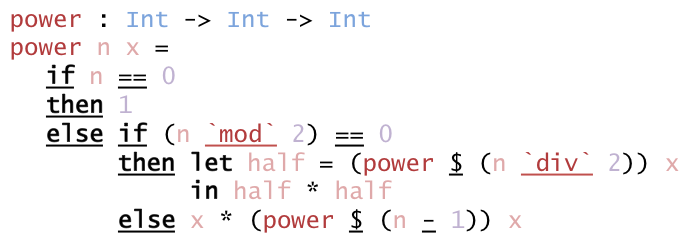
\includegraphics[scale=0.5]{Figures/PowerAnnotated.png}
\end{center}
\caption{Two-level syntax annotated version of \ttdec{power} function, where underlined operations are static}
\label{fig:powan}
\end{figure}

Figure~\ref{fig:powan} shows an annotated version of \ttdec{power} where \ttvar{n} is assumed to be provided statically.
The annotation shows what will be reduced after a value for \ttvar{n} is provided, and as can be seen in the specialised version (see Figure~\ref{fig:powspec}) there
are no traces left of expression marked as static in the residual program.
If \ttvar{n} is to be provided at runtime, it is usually possible to forget the binding-time annotations and execute all of \ttdec{power} dynamically.


\section{Constructor specialisation}
\label{sec:ConstructorSpecialisation}
The previous sections focused mostly on partial evaluation as a way of optimising code, however \textcite{Mogensen:1993:CS:154630.154633} and \textcite{Dussart:1995:PCS:215465.215554} suggest that partial evaluation is also a useful technique to optimise data.
The core idea is to specialise constructors in the same vein as specialising functions, or rather specifically, create new constructors as alternatives of algebraic datatypes where the statically provided input is fixed (or perhaps completely erased).

\subsection{Example: Serialisation to S-expressions}
\label{sub:Example:SerialisationtoS-expressions}

Assume there is a program that serialises an association list to an S-expression and is specialised with regards to a specific schema where it is either the name and age of a person or the name of a department.
Figure~\ref{fig:conspec} shows how a reasonable result could look like after using ordinary partial evaluation techniques.

\begin{figure}[ht]
\begin{center}
    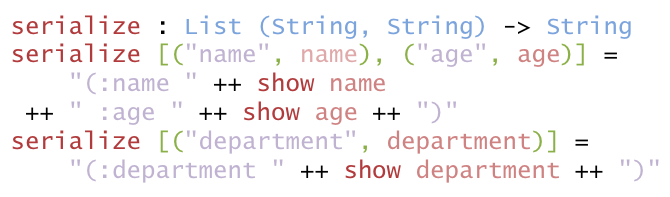
\includegraphics[scale=0.5]{Figures/ConstructorSpecialisation.png}
\end{center}
\caption{A program for serialisation \ttdec{serialize}, specialised using classic techniques with regards to a specific schema}
\label{fig:conspec}
\end{figure}

There are however still some drawbacks with such program: it requires pattern matching on nested constructors, and does multiple string comparisons, both of which are potentially very time consuming.
Yet, much of the data is statically specified, so it seems that there is still room for improvement.
Luckily, constructor specialisation permits specialisation of data by creating suitable constructors in a suitable datatype.
Figure~\ref{fig:conspecdata} shows how new constructors are created in a datatype \tttype{Schema} such that all static data is eliminated, and two suitable constructors are created: \ttconstructor{Person} and \ttconstructor{Department}
\footnote{For ease of reading, the naming is prettified compared to what automated constructor specialisation would generate}.
After constructor specialisation, now the only comparison necessary is comparing tags of datatypes, something which should be much more efficient than the old solution.

\begin{figure}[ht]
\begin{center}
    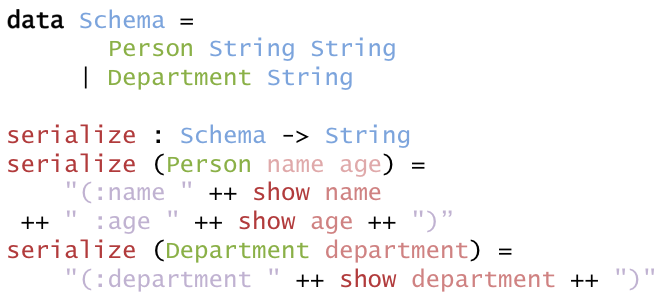
\includegraphics[scale=0.5]{Figures/ConstructorSpecialisationData.png}
\end{center}
\caption{A constructor specialised version of \ttdec{serialize}}
\label{fig:conspecdata}
\end{figure}

\subsection{Algorithm for specialising constructors}
\label{sub:Algorithm for specialising constructors}
\textcite{Dussart:1995:PCS:215465.215554} presents a step-by-step algorithm for performing constructor specialisation that has multiple advantages compared to the original one presented in \textcite{Mogensen:1993:CS:154630.154633}.
One advantage is that it specialises constructors in a polyvariant fashion, which means that specialisation of one datatype can create multiple new datatypes.
Another advantage is that it only requires one pass for calculating the fix-point calculations necessary in order to create new suitable types.
The algorithm consists of three phases: finding a minimal pattern that describes the occurrences of constructors with static values, generating the necessary code operating on such values
and finally creating suitable datatypes to hold the specialised constructors.

\paragraph{A grammar of datatypes}
\label{par:Findingaminimalgrammar}
The first phase of the algorithm is to find a possibly recursive pattern or \textit{grammar} that describes what particular sets of constructors occur in the same expression
at given program points. For the example presented in Figure~\ref{fig:conspec}, the final grammar would look like something shown in Example~\ref{exmp:grammarspec} (in BNF style notation).

\setlength{\grammarparsep}{12pt plus 1pt minus 1pt} % increase separation between rules
\setlength{\grammarindent}{12em}
\begin{exmp}
  \begin{grammar}

    <string> ::= \ldots

    <schema> ::= [("name", <string>), ("age", <string>)]
    \alt [("department", <string>)]
  \end{grammar}
  \label{exmp:grammarspec}
\end{exmp}

The grammar is extracted by analysing the code structure for where data is constructed and suitably combining such data, e.g. having alternatives in the grammar where there are \texttt{\textbf{case}}-expressions.
To avoid non-termination while partially evaluating, the analysis tries to generalise (that is specify as dynamic) places where there occur recursive references to the same datatype.
The effect of that is that non-terminals in the grammar might be defined recursively, which closely mimics the structure of inductive datatypes.
Following extraction of the grammar, fix-point computation techniques inspired by \textcite{Jones:1986:DFA:512644.512672} are used to find a minimal function graph that depends on such grammar.
%A bit vague

\paragraph{Code generation}
\label{par:Code generation}
The second phase uses the minimal function graph found in the first one to construct specialised versions of functions.
This happens by traversing the graph and specialising each function as normal, recursively rebuilding expressions from specialised versions.
\texttt{\textbf{case}}-expressions are handled specially during code generation in order to accommodate the specialised datatypes, and therefore they are restructured, adding new branches, such that they fit the extracted grammar.

\paragraph{Defining suitable types}
\label{par:Defining suitable types}
The final phase is to group the newly generated specialised constructors into suitable type definitions.
This is done in order for the residual program to be valid (type correct) and the compiler can perform other datatype optimisations.
The process prestented is simple: it starts with all constructors being in their own datatype, and merges datatype as necessary when a program dependens on values from either datatype.

\chapter{Levitating Idris}
\label{cha:LevitatingIdris}

\section{Creating descriptions from ordinary datatype declarations}
\label{sec:Creating descriptions from ordinary data declarations}
The description datatype \tttype{Desc} described in Chapter~\ref{cha:GenericProgramming} presents the necessary plumbing to perform generic programming.
However, creating described types required a lot of boilerplate code, requiring labels, descriptions and aliases to be manually written out using the provided low-level constructs.
It would be much better if the compiler could generate the necessary descriptions and aliases from ordinary datatype declarations, since that would provide a more high-level overview of the datatype that mimics what the programmer normally writes.
This section highlights my effort on extending the Idris language with constructors to make it simpler to work with described types.

\subsection{High-level overview}
\label{sub:High-level overview}
To ease the usage of described types in Idris I have added three new language constructs: an annotation on datatypes \texttt{\textbf{\%described}} and two build in operations \texttt{\textbf{labels\_for}} and \texttt{\textbf{desc\_for}}.
The \texttt{\textbf{\%described}} annotation is used before a datatype declaration (see Figure~\ref{fig:natdeclgen}), and specifies to the compiler that it should generate functions relevant to working with described types.
The functions that are generated are in similar style to the ones presented in Sections~\ref{sub:ADescriptionforDatatypes}--\ref{sub:Example:Constructing Vectors}, and represents: the constructor labels of type \tttype{CEnum} for the datatype, the description of type \tttype{Desc} for the datatype, an alias for the described version of the datatype and relevant aliases for its constructors.

\begin{figure}
\begin{center}
    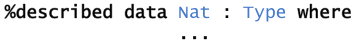
\includegraphics[scale=0.5]{Figures/NatDeclarationGen.png}
\end{center}
\caption{An annotation \texttt{\textbf{\%described}} for generating descriptions from declarations}
\label{fig:natdeclgen}
\end{figure}

To access the generated constructor labels for a particular datatype, the \texttt{\textbf{labels\_for}} operation is used.
For example, to access the generated version of \ttdec{VecCtors} from Figure~\ref{fig:vectctors}, one must use \texttt{\textbf{labels\_for}}~\tttype{Vec}.
Similarly \texttt{\textbf{desc\_for}} is used to access the generated description for a datatype, \textit{e.g.}, \texttt{\textbf{desc\_for}}~\tttype{Vec} returns the equivalent value of \ttdec{VecDesc} from Figure~\ref{fig:descvec}.
The type and constructor aliases are chosen to match the signature and name of the datatype to be described, similarly to how it was done in Section~\ref{sub:Example:Constructing Vectors}.

\subsection{Algorithms for generation}
\label{sub:Algorithms for generation}
When a user asks the compiler to generate relevant functions for working with described types (using \texttt{\textbf{\%described}}), then the compiler performs generation of four types of functions:
one representing the constructor labels of the datatype, one representing the description of the datatype, one representing a type alias based on the description and for each constructor of the datatype, a function that constructs an isomorphic value of the described type.
The following paragraphs describes informally how each of these types of functions are generated from the perspective of the compiler.
The main part of the Haskell function that generates these functions can be seen in Appendix~\ref{cha:Generation function}.\footnote{Due to time constraints, the current version of the function only supports datatypes without parameters and indices.}

\subsubsection{Generation of labels}
\label{ssub:Generation of labels}
The first part of what is generated is a value containing a list of all the constructor names of the target described datatype.
Since all the constructor names are represented internally as strings by the compiler, this step simply involves creating a new clause of type \tttype{CEnum} and assigning it a list where all the constructor names are converted to string literals.

\subsubsection{Generation of descriptions}
\label{ssub:Generation of descriptions}
The second part of what is generated is a value containing the description of the target described datatype.
The algorithm described in Algorithm~\ref{alg:gendescd} works by traversing the Idris AST, finally producing a new declaration which contains the description.

\begin{alg}
  Generating descriptions for datatypes
  \begin{enumerate}
    \item Given a division of parameters and indices create a fitting type signature for the description
       \begin{enumerate}
         \item For parameters quantify those over the whole description value
         \item Additionally quantify a \ttdec{CLabel} and dependent \tttype{Tag} value, to use for representing the description as one with constructor tags
         \item For indices, they are first ``uncurried'' in a dependent pair, and then the whole dependent pair is passed to the tagged description type \tttype{TaggedDesc} as index
         \item[] That is, the description for \tttype{D}\texttt{:}\texttt{(}\ttvar{x$_1$}\texttt{:}\ttvar{a$_1$}\texttt{)}\texttt{\ldots}\texttt{(}\ttvar{x$_n$}\texttt{:}\ttvar{a$_n$}\texttt{)}\texttt{~->~}\texttt{(}\ttvar{y$_1$}\texttt{:}\ttvar{i$_1$}\texttt{)}\texttt{\ldots}\texttt{(}\ttvar{y$_n$}\texttt{:}\ttvar{i$_n$}\texttt{)}\texttt{~->~}\tttype{Type} 
           the signature of the description becomes \texttt{(}\ttvar{x$_1$}\texttt{:}\tttype{a$_1$}\texttt{)}\texttt{~->~}\texttt{\ldots}\texttt{~->~}\texttt{(}\ttvar{x$_n$}\texttt{:}\tttype{a$_n$}\texttt{)}\texttt{~->} \ttdec{TaggedDesc}~\texttt{(\textbf{labels_for}}~\tttype{D}\texttt{)}~\tttype{(}\ttvar{y$_1$}\texttt{:}\ttvar{i$_1$}\tttype{**}\texttt{\ldots}\tttype{**}\ttvar{y$_n$}\texttt{:}\ttvar{i$_n$}\tttype{)} where \ttvar{a$_j$} is the type of a parameter and \ttvar{i$_k$} is the type of an index
       \end{enumerate}
     \item Create a fitting clause to calculate the description where all parameters \ttvar{x$_1$}\texttt{\ldots}\ttvar{x$_n$} are given as arguments to that clause such that the right-hand side can access them
     \item For the right-hand side calculate the $\pi$ value associated with description given the constructors and apply \ttdec{switchDesc} to that
       \begin{enumerate}
         \item To calculate the $\pi$ value for datatype, iterate through the constructors such that for each constructor \ttvar{c$_j$}:
         \begin{enumerate}
           \item Create a new pair where the first component is the description for \ttvar{c$_j$} and the second component is the descriptions for the rest of the constructors ending with \ttconstructor{()}
           \item To calculate the description for \ttvar{c$_j$}, iterate through all its arguments:
           \begin{enumerate}
             \item If the argument is recursive, use the relevant constructor for recursion, either \ttconstructor{Rec} or \ttconstructor{HRec}, and apply it to the index values ``uncurried'' in a dependent pair
             \item[] For example, for an argument \tttype{D}~\ttvar{y$_1$}~\texttt{\ldots}~\ttvar{y$_n$}\texttt{~->~\ldots} use \ttconstructor{Rec}~\ttconstructor{(}\ttvar{y$_1$}\ttconstructor{**}\texttt{\ldots}\ttconstructor{**}\ttvar{y$_n$}\ttconstructor{)}~\texttt{\ldots}
             \item Otherwise if the argument is not recursive, use \ttconstructor{Arg}
             \item[] For example, for an argument \texttt{(}\ttvar{x}\texttt{:}\tttype{A}\texttt{)}\texttt{~->~\ldots} use \ttconstructor{Arg}~\tttype{A}~\texttt{(\textbackslash}\ttvar{x}\texttt{=>\ldots)}
             \item Finally, when the resulting type is reached use \ttconstructor{Ret} applying it to the expected indices in the same way as when working with recursive arguments
           \end{enumerate}
         \end{enumerate}
       \end{enumerate}
  \end{enumerate}
  \label{alg:gendescd}
\end{alg}

After the description is generated it is elaborated by the Idris compiler to ensure that the generated code is correct.
If the description is elaborated successfully, the user can then access it using the \texttt{\textbf{desc\_for}} operation as described in Section~\ref{sub:High-level overview}.

\subsubsection{Generation of aliases}
\label{ssub:Generation of aliases}
The generation of a type alias for a datatype \tttype{D} is simple.
First, create a new declaration with the same name \ttdec{D} and type signature of the datatype. 
Then, the result of \ttdec{D} is \ttdec{TData} applied to the description for that datatype \texttt{\textbf{desc\_for}}~\tttype{D}, adjusting for application of parameters and indices to fit the expected form.
That is, the values of the parameters must be provided to the description to get a value of type \ttdec{TaggedDesc}~\texttt{(\textbf{labels\_for}}~\tttype{D}\texttt{))}~\tttype{(}\ttvar{y$_1$}\texttt{:}\ttvar{i$_1$}\tttype{**}\texttt{\ldots}\tttype{**}\ttvar{y$_n$}\texttt{:}\ttvar{i$_n$}\tttype{)}; then
\ttdec{TData} is applied to that value and in addition the values of the indices which are packed together in a dependent pair yielding a value of type \tttype{Type} as required.

Generating constructor aliases requires a bit more effort than with type aliases, but still follows a step-by-step process.
The first thing is to enumerate all constructors, incrementally assigning each one a number (starting from \ttliteral{0}) which is used to calculate the corresponding \tttype{Tag} value.
Similarly to how type aliases were generated, a new declaration is then created for each constructor \ttconstructor{C} with the corresponding name \ttdec{C} and type signature.
The only difference is that recursive arguments in the type signature are changed to use the described version of the datatype using the generated type alias.
The result of \ttdec{D} is the application of \ttconstructor{Con} to an expression formed of right-nested dependent pairs that represent the synthesised version of the description for the datatype of \ttconstructor{C}.
That is, the nested dependent pairs contain the constructor label, followed by the constructor tag which is calculated from the assigned number, then followed by the arguments of the constructor
and finally ending with the value \ttconstructor{Refl}.

\section{Parametric extension to descriptions}
\label{sec:Parametricextensiontodescriptions}

While it was possible to describe parametrised datatypes using the description presented in Chapter~\ref{cha:GenericProgramming}, it was not possible to distinguish
between values of the parameter and other values after instantiating the parameter.
Therefore, some of the algorithms which dependent upon the knowledge of where a particular parameter is such as the functorial map,
cannot be implemented in a generic fashion.
Since it would be desirable to create such algorithms, a suitable description which has a built-in encoding of parameters must be created.
Section~\ref{sub:The parametricity of parameters} investigates some of the existing notions of what parameters are, and Section~\ref{sub:Parametrically extending the description} shows a new description which supports
the parametric notion of parameters.

\subsection{The parametricity of parameters}
\label{sub:The parametricity of parameters}
What is a parameter?
In an environment with dependent types, such simple question can lead to many more answers than one would initially expect!
While almost all agree on that the type \tttype{Vec}~\ttvar{a}~\ttvar{n} is parametrised by \ttvar{a} and indexed by \ttvar{n}, there has been seemingly less agreement on what a parameter is in general.
The issue is probably due to the different things the different types of ``parameters'' are used for, and sometimes the different types overlap which makes the word \textit{parameter} overloaded.
I will in the following sections present different definitions of what a parameter actually is, explain the rationale of their definition and show where they don't agree.

\subsubsection{Parameters as eliminator quantifiers}
\label{ssub:Parameters as eliminator quantifiers}
One notion of a parameter is presented by \textcite{Dybjer97inductivefamilies}, and is the one that is actually implemented in Idris\,\autocite{brady2013idris}.
The notion is defined in terms of how a parameter appears in the elimination rule for a particular datatype, where it is expected that parameters appear first such that they are quantified over the complete elimination rule.

\begin{figure}[ht]
\begin{center}
    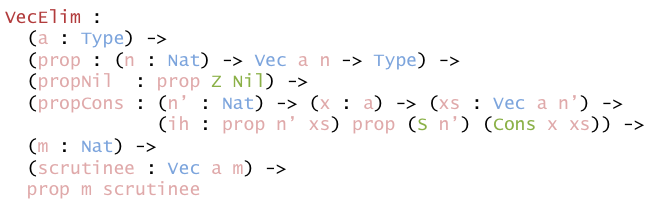
\includegraphics[scale=0.5]{Figures/VectorElim.png}
\end{center}
\caption{Elimination rule for \tttype{Vec}}
\label{fig:vecelim}
\end{figure}

Since parameters are quantified over the elimination rule, it is ensured that they are constant relative to the property to be eliminated, \textit{i.e.}, they do not change depending on the value that may be provided as scrutinee.
Figure~\ref{fig:vecelim} shows the elimination rule for \tttype{Vec}, where it can be observed that \ttvar{a} is quantified over the whole expression and thus parameteric,
while \ttvar{n} changes in the property to be eliminated \ttvar{prop} and is therefore considered an index.

A restriction that is necessary to ensure that parameters are quantified correctly in the elimination rule, is that the parameter should appear uniformly in all of the constructors result type or recursive arguments.
This rules out data structures such as the one presented in Figure~\ref{fig:nestedlist} to be considered parametric in this system, since the argument to the recursive argument of \ttconstructor{Cons} is different
than in the rest of the structure.

\subsubsection{Parameters as terms with parametricity}
\label{ssub:Parameters as terms with parametricity}
Another notion of a parameter which is presented by \textcite{bernardy2010parametricity}, is that it is a type argument which exhibits parametricity\,\autocite{DBLP:conf/ifip/Reynolds83,Wadler89theoremsfor}.
A type argument exhibits parametricity if the same relations in the datatype is satisfied independently of which value is provided; that is, one should not be able to inspect or constrain the value of a parameter (using e.g. propositional equality).
Figure~\ref{fig:nestedlist} shows a nested datatype\,\autocite{bird1998nested} \tttype{NList}, which is parameteric even though \ttvar{a} does not appear uniformly in the datatype declaration.
The reason that \ttvar{a} is still considered parameteric, is because the recursive argument uses \textit{functorial composition}.
With functorial composition, recursive arguments can use parameters in a non-uniform fashion as long as it does not change parametericity and preserves the expected relations.
In the \tttype{NList} example, the \tttype{NList}~\tttype{(}\ttvar{a}\tttype{,}\ttvar{a}\tttype{)} argument can be seen as a composition of \tttype{NList} with the homogenous pair type \texttt{\textbackslash}\ttvar{p}\texttt{=>}\tttype{(}\ttvar{p}\tttype{,}\ttvar{p}\tttype{)} which itself satisfies the necessary parametricity requirements.

\begin{figure}[ht]
\begin{center}
    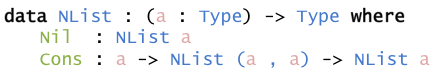
\includegraphics[scale=0.5]{Figures/NestedList.png}
\end{center}
\caption{The nested datatype \tttype{NList}}
\label{fig:nestedlist}
\end{figure}

Parametricity of type arguments is necessary to correctly implement useful declarative function, such as those that are methods of the \tttype{Functor}, \tttype{Traversable} and \tttype{Foldable} type classes from Haskell.
If constraints were made based on the type argument of the datatype, it wouldn't be possible to satisfy the associated laws of these type classes and possibly not even provide an implementation that can type check.

\subsubsection{Parameters as uniform indices}
\label{ssub:Parameters as uniform indices}
The last notion of a parameter is the one used in Agda\,\autocite{norell2009dependently} which only requires that parameters are uniform in the resulting type of constructors.
This allows the creation of more expressive datatypes, and can encompass both parametric parameters and parameters which are quantified uniformly over eliminators however it does not ensure either of these properties.
While this provides more freedom for the user to decide how to structure datatypes, it makes it harder to see what the correspondence there is between a parameter and the semantic properties it imposes.

\begin{figure}[ht]
\begin{center}
    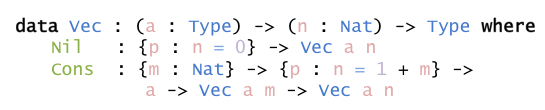
\includegraphics[scale=0.5]{Figures/VectorAlternativeDeclaration.png}
\end{center}
\caption{Alternative definition of \tttype{Vec} using equality constraints}
\label{fig:altvecdecl}
\end{figure}

For example, Figure~\ref{fig:altvecdecl} shows a datatype where both \ttvar{a} and \ttvar{n} are uniform in the result and which could accepted as a \citeauthor{norell2009dependently}-style parameter.
However, the arguments in this definition are neither parametric nor uniform and therefore does not fit into another definition of parameters.


\subsection{Parametrically extending the description}
\label{sub:Parametrically extending the description}
One suggestion on how to ensure the parametricity of parameters was made by \textcite{bernardy2011theory}.
It was suggested that whenever a parameter was bound and parametricity was needed, one could provide an additional argument
the \textit{witness} which proved that such parameter was parametric.
However such suggestion could be hard to work with in practical generic programming and instead this section would focus on providing
an encoding that is conservative in a way that disallows non-parametric use of parameters but is still able to express many interesting datatypes.

\subsubsection{Explicit parameters}
\label{ssub:Explicit parameters}

\begin{figure}[ht]
\begin{center}
    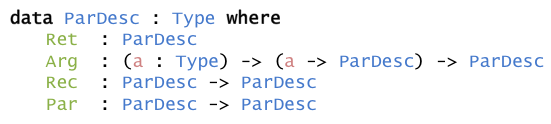
\includegraphics[scale=0.5]{Figures/ParDescriptionType.png}
\end{center}
\caption{A description for parametrised types}
\label{fig:pardesc}
\end{figure}

Figure~\ref{fig:pardesc} presents a description
\footnote{\ttconstructor{HRec} is omitted for presentation purposes, but can be added in the same style as presented in Chapter~\ref{cha:GenericProgramming}} 
akin to the one presented in Figure~\ref{fig:simpldescdatatype}
except a new constructor \ttconstructor{Par} which is inspired by an encoding in \textcite{benke2003universes} is added.
The constructor \ttconstructor{Par} represents an argument of the provided parameter in the datatype to be described.

\begin{figure}[ht]
\begin{center}
    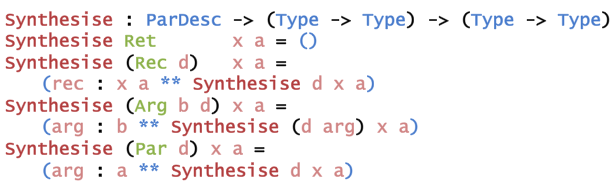
\includegraphics[scale=0.5]{Figures/ParSynthesising.png}
\end{center}
\caption{Synthesising an ordinary type from \tttype{ParDesc}}
\label{fig:parsynth}
\end{figure}

In order, to convert the newly presented description to an ordinary datatype a suitable \ttdec{Synthesise} function is declared.
The function looks mostly the same as the one presented in Chapter~\ref{cha:GenericProgramming}, the described type is now of type \tttype{Type}\texttt{ -> }\tttype{Type}
and an additional clause for \ttconstructor{Par}.
The clause for \ttconstructor{Par} produces a dependent pair similar to most other clauses, where the first component has to be an argument of the provided parameter as expected
and the second component is the type synthesised from the rest of the description.
Since it is not possible to dependent on the type nor values of parameters in the presented encoding, parametericity is ensured by construction.
However, some expression power is lost in return since it is not possible to have complex arguments of other types that uses these parameters.

\subsubsection{Supporting functorial composition}
\label{ssub:Supporting functorial composition}
In Section~\ref{sub:The parametricity of parameters} it was stated that parameters in nested datatypes were parameteric
because they were composed in a functorial fashion.
It would be therefore desirable to be add such ability to the presented description, since it would increase the level of expression.

\begin{figure}[ht]
\begin{center}
    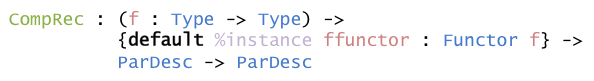
\includegraphics[scale=0.5]{Figures/ParDescriptionTypeExtended.png}
\end{center}
\caption{Adding support for describing functorial composition}
\label{fig:pardescex}
\end{figure}

Figure~\ref{fig:pardescex} shows the addition of the \ttconstructor{CompRec} which represents a nested recursive argument of a datatype.
The first argument of the constructor \ttvar{f} is the type to be functorially composed onto the parameter, and must therefore be a function that accepts the parameter
and returns a type.
To ensure that \ttvar{f} acts functorially, an additional argument \ttvar{ffunctor} must be given.
This variable \ttvar{ffunctor} provides the \tttype{Functor} type class instance for \ttvar{f}, and the argument is written such way that it tries to implicitly resolve the instance via the built-in type class resolution mechanism.
Finally the last argument is the rest of the description for the datatype described.

\begin{figure}[ht]
\begin{center}
    \includegraphics[scale=0.5]{Figures/ParSynthesisingExtended.png}
\end{center}
\caption{Transforming \ttconstructor{CompRec} to a type}
\label{fig:parsynthex}
\end{figure}

Converting \ttconstructor{CompRec} to an ordinary type is mostly similar to converting ordinary recursive arguments \ttconstructor{Rec} (see Figure~\ref{fig:parsynthex}).
The only difference is that \ttvar{f} must be applied to the parameter first before applying the described version of the type.
It is perhaps clearest here why it is called functorial composition, since \ttvar{x}~\texttt{(}\ttvar{f}~\ttvar{a}\texttt{)} is equivalent to \texttt{(}\ttvar{x}~\texttt{.}~\ttvar{f}\texttt{)}~\ttvar{a} which uses
the ordinary function composition operator ``\texttt{.}''.

\begin{figure}[ht]
\begin{center}
    \includegraphics[scale=0.5]{Figures/NestedListDescription}
\end{center}
\caption{Described version of \tttype{NList}}
\label{fig:nlistdesc}
\end{figure}

As an example of a description for a nested datatype, please take a look at Figure~\ref{fig:nlistdesc}.
The figure shows the description for \tttype{NList} from Figure~\ref{fig:nestedlist}, and the most interesting
part is the application of \ttconstructor{CompRec}.
In this context it is applied to a functor \ttdec{PairP}, which represents the same type as \texttt{\textbackslash}\ttvar{p}\texttt{=>}\tttype{(}\ttvar{p}\tttype{,}\ttvar{p}\tttype{)} from Section~\ref{sub:The parametricity of parameters}.
To typecheck this application of \ttconstructor{CompRec} there must be a \tttype{Functor} instance for \ttdec{PairP}, however as can be observed in the figure it doesn't have to be provided explicitly.

\subsubsection{Conversion to ordinary descriptions}
\label{ssub:Conversion to ordinary descriptions}

Descriptions for parametrised datatypes can be converted to ordinary description using a simple step-by-step process (see Figure~\ref{fig:pardesctodesc}).
The result type must be indexed by \tttype{Type}, because recursion expressed by \ttconstructor{CompRec} is not uniform and therefore can't be quantified uniformly over the whole description.
Since the converted description would hold the same data as the provided input description, it allows generic descriptions written for ordinary descriptions to be reused.
In fact, converting the description and then performing synthesis should yield isomorphic data, which means that \ttdec{Synthesise} only needs to be implemented for ordinary descriptions.

\begin{figure}[ht]
\begin{center}
    \includegraphics[scale=0.5]{Figures/ParDescriptionConversion.png}
\end{center}
\caption{Converting \tttype{ParDesc} to ordinary indexed \tttype{Desc}}
\label{fig:pardesctodesc}
\end{figure}

While \tttype{ParDesc} and \tttype{Desc} were presented as two separate datatypes for readability purposes, they can be in fact combined.
The only thing that adds complexity is that the presence or absence of parameters must be accounted for at all stages, and further generalisation towards arity-generic programming requires some advanced fiddling with the type system.


\section{Proposed Improvements}
\label{sec:ProposedImprovements}

\subsection{Any practical type theory permits forgetting unused dependencies}
\label{sub:Any practical type theory permits forgetting unused dependencies}


\chapter{Practical examples}
\label{cha:PracticalExamples}

\section{Generic algorithms for deriving type class instances}
\label{sec:Genericalgorithmsforderivingtypeclassinstances}

\subsection{Specifying the necessary constraints}
\label{sub:Specifying the necessary constraints}

For many type classes, implementing them for a complex datatype sometimes require an implementation of the type class for its subparts.
For example, to pretty a list of items it is required that there is a way to print each individual element.

\begin{figure}[ht]
\begin{center}
    \includegraphics[scale=0.5]{Figures/ConstrainingTypeclasses.png}
\end{center}
\caption{A function that calculates type class constraints for a single parameter type class}
\label{fig:constrclass}
\end{figure}

Figure~\ref{fig:constrclass} shows a function \ttdec{Constraints1} which can be used to calculate type class constraints
for a type class \ttvar{class} that takes a simple parameter of type \tttype{Type}, given a description of type \tttype{Desc}.
The function works mostly by iterating over the description type and specifies that each external data member with description \ttconstructor{Arg}
must have an implementation of the provided type class.
The only other interesting case is \ttconstructor{HRec}, where the false type \tttype{\_|\_} is required.
The false type makes it impossible to fulfil the constraints for a datatype using \ttconstructor{HRec}, and is used intentionally to avoid implementing algorithms using descriptions of that form.
This is because it is generally hard to implement arbitrary algorithms like decidable equality on functions which \ttconstructor{HRec} symbolises.

\subsection{Pretty printing}
\label{sub:Pretty printing}
One of the most commonly used and automatically derived operations on datatypes is pretty printing.
Therefore, this function suits well as an introductory example on how a generic algorithm using the presented implementation of description
look like.

\begin{figure}[ht]
\begin{center}
    \includegraphics[scale=0.5]{Figures/GenericShow.png}
\end{center}
\caption{Generically pretty printing a described type}
\label{fig:showgen}
\end{figure}

The algorithm for generic pretty printing \ttdec{gshow} is shown in Figure~\ref{fig:showgen}, and follows well the informal algorithm presented in Example~\ref{exmp:prettyprint}.
The type signature of the \ttdec{gshow} might look a bit daunting at first, but the only major difference from ordinary pretty printing is that it requires not just data but also the associated description
and some constraints on its subcomponents to be able to pretty print them.
The function first prints the name of the input constructor, and then calls a function \ttdec{gshowd} which pretty prints the individual constructor arguments according to the provided description.

\begin{figure}[ht]
\begin{center}
    \includegraphics[scale=0.5]{Figures/GenericShowDesc.png}
\end{center}
\caption{Iterating through the description and pretty printing individual components}
\label{fig:showgendesc}
\end{figure}

The function \ttdec{gshowd} shown in Figure~\ref{fig:showgendesc}, iterates through the arguments of the input constructor.
If there we reach the end of the constructor (having description \ttconstructor{Ret}), the empty string is printed.
If it is a recursive argument, the generic show \ttdec{gshow} is called again with the description for the whole datatype, parenthesised if necessary; then the rest of the constructor arguments are printed.
Otherwise if it is an ordinary argument, the associated \ttdec{show} method is called using the instance provided from the constraints, again parenthesised if necessary, and then the rest of the of the constructor arguments are printed.
Finally, if a higher-order recursive argument is met it is dismissed using \ttdec{absurd} since it should not be possible to reach this case because the constraints require a value of type \tttype{\_|\_}.


\subsubsection{Example: Implementing \tttype{Show} for the described type \ttdec{Pair}}
\label{ssub:Example:ImplementingShowforPairs}
As an example on how to use the generic pretty print function \ttdec{gshow} to implement the \ttdec{show} method of \tttype{Show} type class for the described type \ttdec{Pair}, see Figure~\ref{fig:showinst}.
The call to \ttdec{gshow} is passed the description \ttdec{PairDesc} and the necesssary constraints \ttdec{pairShowConstrs} which definition is shown in Figure~\ref{fig:showconstrs}.
To create the constraints structure, one simply has to create a tuple to match the type required by \ttdec{Constraints1} and then call \ttliteral{\%instance} the right places.
The \ttliteral{\%instance} expression is evaluated at compile time, and allows Idris to perform type class resolution returning the associated instance for the target type class.

\begin{figure}[ht]
\begin{center}
    \includegraphics[scale=0.5]{Figures/GenericShowConstraints.png}
\end{center}
\caption{Constraints necessary to implement \tttype{Show} for \ttdec{Pair}}
\label{fig:showconstrs}
\end{figure}

The \tttype{Show} constraints for \ttdec{Pair} are easy to create, and are almost on the verge of being boilerplate.
In fact calculating the constraints for other single-parameter type classes have almost the exact same structure.
The issues however lies with that Idris cannot do type class resolution for any type class \ttvar{c}, and therefore it is impossible to make
a function that calculates these constraints (since it would not be able to type check).
There could be two solution to such issue: one would be to create a macro system for Idris which only type checks the expression after it is instantiated with the right type class, and another
would be to create a suitable tactic that calculates such constraints at compile time when needed.
Since these solutions would require some effort which is beyond the scope of this project, they are considered to be future work.

\begin{figure}[ht]
\begin{center}
    \includegraphics[scale=0.5]{Figures/GenericShowInstance.png}
\end{center}
\caption{Creating a \tttype{Show} instance for \ttdec{Pair} using the generic \ttdec{gshow}}
\label{fig:showinst}
\end{figure}

\subsection{Decidable equality}
\label{sub:Decidable equality}
Something which is a bit more interesting to do generically than pretty printing is decidable equality, since that usually
requires handling a quadratic number of cases relative to number of constructors and \textbf{in addition} writing a significant number of associated lemmas.
However, before implementing decidable equality for described types, I will start by implementing it for \tttype{Tag} to make it easier for the user to satisfy
the necessary constraints.

\begin{figure}[ht]
\begin{center}
    \includegraphics[scale=0.5]{Figures/TagDecEqLemma1.png}
\end{center}
\caption{Lemma specifying that \ttconstructor{TZ} is not equal to \ttconstructor{TS}}
\label{fig:taglem1}
\end{figure}

To implement decidable equality for \tttype{Tag}, a couple of lemmas are necessary.
The first necessary lemma \ttdec{lemma\_tz\_not\_ts} is shown in Figure~\ref{fig:taglem1} which shows that the different constructors of \tttype{Tag},
\ttconstructor{TZ} and \ttconstructor{TS} are different.

\begin{figure}[ht]
\begin{center}
    \includegraphics[scale=0.5]{Figures/TagDecEqLemma2.png}
\end{center}
\caption{Lemma proving the injectivity of \ttconstructor{TS}}
\label{fig:taglem2}
\end{figure}

The second necessary lemma to prove is the injectivity of the constructor \ttconstructor{TS} (see Figure~\ref{fig:taglem2}).
That is, if given two values of constructor \ttconstructor{TS} which are equal, then it is possible to show that their inner \tttype{Tag} arguments
are equal.

\begin{figure}[ht]
\begin{center}
    \includegraphics[scale=0.5]{Figures/TagDecEqLemmaInstance.png}
\end{center}
\caption{\tttype{DecEq} instance for \tttype{Tag}}
\label{fig:tagdeceqinst}
\end{figure}

Given the necessary lemmas, it should now be possible to implement the \tttype{DecEq} instance for \tttype{Tag}.
The cases are straightforward: if both constructors are \ttconstructor{TZ} then they are always equal, if they differ then they are not equal
and the \ttdec{lemma\_tz\_not\_ts} (or its symmetric version) is used as evidence, and finally if both constructors are \ttconstructor{TS} then they are equal
if their inner tags are equal, otherwise they are not and the injectivity lemma is used to compose proof.

Now, that there is a suitable implementation of decidable equality for tags, it is possible to implement the generic version of decidable equality.
Similarly to the implementation for tags, a few injectivity lemmas are also needed for the generic version of decidable equality: 
one for the injectivity of \ttconstructor{Con}, and two for the injectivity of dependent pairs (which is the type that \ttdec{Synthesise} converts most descriptions to).

\begin{figure}[ht]
\begin{center}
    \includegraphics[scale=0.5]{Figures/GenericDecEqLemma1.png}
\end{center}
\caption{Lemma proving that \ttconstructor{Con} is injective}
\label{fig:dglem1}
\end{figure}

The injectivity lemma for \ttconstructor{Con} is shown in Figure~\ref{fig:dglem1}.
It shows that given that two described types of type \tttype{Data} are equal, then the contained data must be equal too.

\begin{figure}[ht]
\begin{center}
    \includegraphics[scale=0.5]{Figures/GenericDecEqLemma2.png}
\end{center}
\caption{Injectivity lemma for the first component of dependent pairs}
\label{fig:dglem2}
\end{figure}

\begin{figure}[ht]
\begin{center}
    \includegraphics[scale=0.5]{Figures/GenericDecEqLemma3.png}
\end{center}
\caption{Injectivity lemma for the second component of dependent pairs}
\label{fig:dglem3}
\end{figure}

The injectivity lemmas for dependent pairs are shown in Figure~\ref{fig:dglem2} and Figure~\ref{fig:dglem3}.
The first lemma states that given that two dependent pairs are equal, then their first components are equal.
The second lemma states the same, but for the second components instead.

The implementation of generic decidable equality is shown in Figure~\ref{fig:deceqgen}.
The type signature is a similar style to the one for generic pretty printing, and requires both the description
and necessary instances of decidable equality for the subcomponents of the datatype.
The implementation is defined such that two described types constructed with \ttconstructor{Con} are equal, if their individual data components (including constructor tag) are equal.
Otherwise if the individual data components are not equal, then the injectivity lemma for \ttconstructor{Con} is composed with the counter-proof to be used as a new counter-proof for inequality.

\begin{figure}[ht]
\begin{center}
    \includegraphics[scale=0.5]{Figures/GenericDecEq.png}
\end{center}
\caption{deceqgen}
\label{fig:deceqgen}
\end{figure}

To check if the individual components are equal or not, the function \ttdec{gdecEqd} is used, which takes as argument the original description and constraints (to use for recursive calls)
in addition to the description and constraints which need to be iterated.
The type signature for \ttdec{gdecEqd} is shown in Figure~\ref{fig:deceqgendescty}.

\begin{figure}[ht]
\begin{center}
    \includegraphics[scale=0.5]{Figures/GenericDecEqDescType.png}
\end{center}
\caption{The type signature of \ttdec{gdecEqd}}
\label{fig:deceqgendescty}
\end{figure}

If the end of the description is reached (\textit{i.e.}, having the description \ttconstructor{Ret}), then two values are always considered to be equal.
The clause for \ttdec{gdecEqd} in the case of \ttconstructor{Ret} is shown in Figure~\ref{fig:deceqgendesc1}.

\begin{figure}[ht]
\begin{center}
    \includegraphics[scale=0.5]{Figures/GenericDecEqDesc1.png}
\end{center}
\caption{Checking that two described types with description \ttconstructor{Ret} are equal}
\label{fig:deceqgendesc1}
\end{figure}

Probably the most interesting case is shown in Figure~\ref{fig:deceqgendesc2} and is when it is an argument which is described (\textit{i.e.}, \ttconstructor{Arg}).
There are two things which are needed to be checked, the equality of argument values themselves and the equality of the rest of the described type.
To the check if that the values of the provided arguments are equal, the provided type class instance from the constraints is used.
If the values are equal then it is possible to proceed checking the rest of the described type, otherwise the \ttdec{lemma\_fst\_injective} lemma is used to compose a counter-proof.
If the rest of the described type is equal then an equality proof can be provided, otherwise the \ttdec{lemma\_snd\_injective} lemma is used to compose a counter-proof.

\begin{figure}[ht]
\begin{center}
    \includegraphics[scale=0.5]{Figures/GenericDecEqDesc2.png}
\end{center}
\caption{Decidable equality for described types with description \ttconstructor{Arg}}
\label{fig:deceqgendesc2}
\end{figure}

The case of recursive arguments (\textit{i.e.}, \ttconstructor{Rec}) is similar to the case of ordinary arguments (see Figure~\ref{fig:deceqgendesc3}).
Since the equality of the recursive argument is independent of the equality of rest of the described type, both equalities can be checked at the same time.
To check the equality of the recursive arguments \ttdec{gdecEq} is called again with the description for the whole type and associated constraints, in addition to the values
of the recursive arguments.
If both the recursive arguments and the rest of the described type are equal than the result is that the data is equal,
otherwise a contra-proof is composed using the necessary lemma.

\begin{figure}[ht]
\begin{center}
    \includegraphics[scale=0.5]{Figures/GenericDecEqDesc3.png}
\end{center}
\caption{Decidable equality for described types with description \ttconstructor{Rec}}
\label{fig:deceqgendesc3}
\end{figure}

Finally, for described types with description \ttconstructor{HRec}, \ttdec{absurd} is used to dismiss the required implementation since the constraints are not satisfiable similar to
how it was dismissed for generic pretty printing (see Figure~\ref{fig:deceqgendesc4}).

\begin{figure}[ht]
\begin{center}
    \includegraphics[scale=0.5]{Figures/GenericDecEqDesc4.png}
\end{center}
\caption{Decidable equality for described types with description \ttconstructor{HRec}}
\label{fig:deceqgendesc4}
\end{figure}

\subsection{Functorial mapping}
\label{sub:Functorial mapping}
One interesting generic algorithm that wouldn't work on described types just using \tttype{Desc} is the generic map function, since it requires
an encoding of parameters.
Therefore, the algorithm is implemented using the version extended with parameters \tttype{ParDesc}.
The actual implementation of generic map \ttdec{gmapp} is shown in Figure~\ref{fig:mapgen}, and simply says that
mapping a described type is simply the same as mapping its individual data components using \ttdec{gmappd}.

\begin{figure}[ht]
\begin{center}
    \includegraphics[scale=0.5]{Figures/GenericMap.png}
\end{center}
\caption{Generic map}
\label{fig:mapgen}
\end{figure}

The function used to map a function on the individual components \ttdec{gmappd} is presented in Figure~\ref{fig:mapgendesc}.
The implementation is straightforward and mostly iterates through the structure applying the generic mapping functions where possible, and the only two interesting cases is the one for value of the parameter type
and for the functorially composed recursion.
When a parameter value (described by \ttconstructor{Par}) is met, then the function to mapped \ttvar{f} is simply applied to that parameter and the mapping continues on the rest of the described type.
For the functorially composed recursive arguments (described by \ttconstructor{CompRec}), there are a couple of steps to be taken.
First, a mapping function \ttdec{map}~\texttt{@\{}\ttvar{mapc}\texttt{\}}~\ttvar{f} for the elements of the composed type is created by calling the associated \ttvar{Functor} instance \ttvar{mapc} for the composed functor \ttvar{g}, which then has the type \ttvar{g}~\ttvar{a}~\texttt{->}~\ttvar{g}~\ttvar{b}.
Thereafter, this mapping function has the right to be provided to the recursive call of \ttdec{gmapp} and the recursive constructor argument can be mapped.
Finally, it is possible to map the rest of the described type.

\begin{figure}[ht]
\begin{center}
    \includegraphics[scale=0.5]{Figures/GenericMapDesc.png}
\end{center}
\caption{Generically mapping the data components of a described type}
\label{fig:mapgendesc}
\end{figure}


\section{Algorithms with purely generic properties}
\label{sec:Algorithms with purely generic properties}
\subsection{Generic tag testing}
\label{sub:Generic tag testing}
One common pattern in the Idris standard library is to check whether a variable is of a particular constructor type, \textit{e.g.},
to get the \ttdec{head} of a list \ttvar{xs} then \ttdec{isCons}~\ttvar{xs} must be true and to use convert a \tttype{Fin} to an integer using \ttdec{fromInteger} then \ttdec{isJust} is used to ensure that the conversion is safe.
Such use-pattern normally requires setting up a new function for each particular constructor, however with the power of generic programming such pattern can be easily generalised into a function.

\begin{figure}[ht]
\begin{center}
    \includegraphics[scale=0.5]{Figures/GenericIs.png}
\end{center}
\caption{Generic tag testing}
\label{fig:isgen}
\end{figure}

Figure~\ref{fig:isgen} shows a function \ttdec{is} which can be used to do generic constructor testing.
The function uses the decidable equality on strings and values of type \tttype{Tag} to test whether a constructor has equal tag to the one provided.
An interesting feature of \ttdec{is} is that it only requires the name of a constructor to be provided explicitly and will find the associated tag using proof search.
This where the way \tttype{Tag} was structured really shines, since the name of the constructor to be found and the list of possible constructors are part of the type signature
there is only one correct solution.
Therefore, the proof search will never produce the wrong result, since that would not be well-typed.

\subsection{Generic if expression}
\label{sub:Generic if expression}
Another interesting function that could be made generically is a generic version of the \texttt{\textbf{if}}-expression.
Normally the \texttt{\textbf{if}}-expression only works with conditions of type \tttype{Bool}, however the function \ttdec{gif} presented in Figure~\ref{fig:ifgen} works with any datatype with at least two constructors.
If the condition provided matches the first constructor of the datatype that had declared it, then the result is the false branch; otherwise the result of the function is the true branch.

\begin{figure}[ht]
\begin{center}
    \includegraphics[scale=0.5]{Figures/GenericIf.png}
\end{center}
\caption{Generic \texttt{\textbf{if}}-expression}
\label{fig:ifgen}
\end{figure}



\section{Scrapping your dependently-typed boilerplate is hard}
\label{sec:Scrappingyourdependently-typedboilerplateishard}
\textit{A version of the Uniplate library for Idris based on} \url{http://community.haskell.org/~ndm/uniplate/} \textit{and} \url{http://www-ps.informatik.uni-kiel.de/~sebf/projects/traversal.html} \textit{.
This is useful for traversing structures in a generic fashion and especially when dealing with small changes in large data structures (such as compiler ADTs)}

\chapter{Optimising Idris for flight}
\label{cha:OptimizingIdrisforFlight}

\section{Specialising constructors for specific types}
\label{sec:SpecialisingConstructorsforSpecificTypes}
\textit{How generalized constructors of described types, are specialised as ordinary data structures.}

\section{Online erasure of unused arguments}
\label{sec:OnlineErasureofUnusedArguments}
\textit{How some type infromation is to be erased at compile time to reduce elaboration overhead. Very hypothetical.}

\section{Static initialization of generic functions}
\label{sec:StaticInitializationofGenericFunctions}
\textit{How algorithms that are dependent on the generic structure of a datatype are optimised. Discuss benefits of having a JIT/Profiling information for future work.}

\chapter{Evaluation}
\label{cha:Evaluation}

\chapter{Discussion}
\label{cha:Discussion}

%\section{Related Work}
%\label{sec:Related Work}
%\begin{enumerate}
  %\item Less is more by Jose Magalhaes
  %\item Uniplate-like function by/everyWhere by Larry Diehl
%\end{enumerate}

\section{Future work}
\label{sec:FutureWork}

\section{Conclusion}
\label{sec:Conclusion}

\printbibliography
\appendix
\chapter{Generation function}
\label{cha:Generation function}
\lstinputlisting[language=Haskell,breaklines=true,numbers=left,caption={Generating relevant functions for working with described types},label={app:gendesc}]{Code/DescriptionGeneration.hs}
\end{document}
